% hubble_om_sensitivity_v7.tex
% Sensitivity of Pantheon+ Hubble-flow H0 to assumed matter density:
% a xi-space and direct refit analysis
% Eric D. Martin — ORCID: 0009-0006-5944-1742
% MNRAS full research article format

\documentclass[fleqn,usenatbib]{mnras}

\usepackage[T1]{fontenc}
\usepackage{newtxtext,newtxmath}
\usepackage{amsmath}
\usepackage{graphicx}
\usepackage{booktabs}
\usepackage{url}

% Allow VAN-style name sorting in bibliography
\DeclareRobustCommand{\VAN}[3]{#2}
\let\VANthebibliography\thebibliography
\def\thebibliography{\DeclareRobustCommand{\VAN}[3]{##3}\VANthebibliography}

%%%%%%%%%%% TITLE PAGE %%%%%%%%%%%

\title[H$_0$ sensitivity to $\Omega_m$ in Pantheon+]{%
  Sensitivity of Pantheon+ Hubble-flow $H_0$ to assumed matter density:
  a $\xi$-space and direct refit analysis}

\author[E.~D.~Martin]{%
  Eric D. Martin\thanks{E-mail: doctor.eric.martin@gmail.com;
  ORCID: 0009-0006-5944-1742}}

\date{Accepted XXX. Received YYY; in original form ZZZ}
\pubyear{2026}

\begin{document}
\label{firstpage}
\pagerange{\pageref{firstpage}--\pageref{lastpage}}
\maketitle

% ---------------------------------------------------------------
% Abstract — target 200–245 words
% ---------------------------------------------------------------
\begin{abstract}
We investigate how much the inferred Pantheon+SH0ES Hubble-flow $H_0$
changes when the assumed matter density is shifted from the SH0ES-like
value $\Omega_m = 0.334$ to the Planck-like value $\Omega_m = 0.315$,
using the public Pantheon+SH0ES catalogue of 1{,}701 SNe~Ia.
We apply two complementary diagnostics.
The first diagnostic employs the horizon-normalised comoving coordinate
$\xi \equiv d_c/d_H$, which is strictly $H_0$-independent in flat
$\Lambda$CDM.
Comparing the SH0ES-like ($\Omega_m = 0.334$, $H_0 = 73.04$
km\,s$^{-1}$\,Mpc$^{-1}$) and Planck-like ($\Omega_m = 0.315$,
$H_0 = 67.4$ km\,s$^{-1}$\,Mpc$^{-1}$) frameworks across all
1{,}671 SNe~Ia, we measure a mean absolute $\xi$-residual of
$\langle|\Delta\xi|\rangle/\langle\xi_\mathrm{mid}\rangle = 0.56$\,\%, a factor
of 15 smaller than the nominal 8.4\,\% $H_0$ fractional gap.
Second, we perform a simplified Cepheid-anchored direct refit in which
the SN absolute magnitude $M$ is fixed from 77 calibrator SNe~Ia with
Cepheid geometric distances, and $H_0$ is re-optimised over
1{,}616 Hubble-flow SNe at fixed $\Omega_m$, using diagonal
distance-modulus uncertainties.
Under this diagnostic, the best-fit $H_0$ shifts by
$\Delta H_0 = -0.22 \pm 0.005$ km\,s$^{-1}$\,Mpc$^{-1}$
(bootstrap $1\sigma$, $N = 1{,}000$, $\mathrm{S/N} = 46$),
corresponding to 3.9\,\% of the nominal 5.64 km\,s$^{-1}$\,Mpc$^{-1}$
SH0ES--Planck central-value gap.
The $\Omega_m$ sensitivity grows monotonically with redshift, from
$|\Delta H_0| = 0.02$ km\,s$^{-1}$\,Mpc$^{-1}$ at $z < 0.03$ to
$0.49$ km\,s$^{-1}$\,Mpc$^{-1}$ at $z > 0.33$ across four
equal-count redshift quartiles.
Both diagnostics indicate that changing $\Omega_m$ across the
SH0ES--Planck range induces only a modest shift in Pantheon+-based
Hubble-flow $H_0$ relative to the nominal central-value gap.
Under this diagnostic framework, the $\Omega_m$ prior difference
contributes ${\lesssim}\,4$\,\% of that gap; the remaining
discrepancy lies outside the component measured here and requires
matched-likelihood analyses with the full covariance matrices of
both experiments.
\end{abstract}

\begin{keywords}
cosmological parameters --- distance scale --- supernovae: general
\end{keywords}

%%%%%%%%%%% BODY %%%%%%%%%%%

% ---------------------------------------------------------------
\section{Introduction}
\label{sec:intro}
% ---------------------------------------------------------------

The discrepancy between early- and late-Universe determinations of the
Hubble constant $H_0$ is among the most scrutinised open problems in
modern cosmology.
The Planck CMB analysis yields
$H_0 = 67.4 \pm 0.5$ km\,s$^{-1}$\,Mpc$^{-1}$
under flat $\Lambda$CDM with $\Omega_m = 0.315 \pm 0.007$
\citep{planck2020}, while the SH0ES Cepheid--supernova distance ladder
measures
$H_0 = 73.04 \pm 1.04$ km\,s$^{-1}$\,Mpc$^{-1}$
from a fit with $\Omega_m = 0.334 \pm 0.018$ \citep{riess2022}.
The fractional gap is ${\sim}\,8.4$\,\%,
corresponding to a statistical significance of approximately
$5\sigma$ when the individual error budgets are taken at face value
\citep{verde2019,divalentino2021,perivolaropoulos2022}.

This discrepancy has motivated a broad programme of observational
cross-checks and theoretical extensions.
Independent $H_0$ measurements from the Tip of the Red Giant Branch
\citep{freedman2019,freedman2021,freedman2024},
megamaser cosmology \citep{pesce2020},
strong-lensing time delays \citep{wong2020,birrer2020},
surface brightness fluctuations \citep{blakeslee2021},
and gravitational-wave standard sirens \citep{abbott2017gw}
yield a range of values that do not uniformly support either the
CMB-based or the Cepheid-based result, although most late-Universe
probes prefer $H_0 \gtrsim 70$ km\,s$^{-1}$\,Mpc$^{-1}$.
On the theoretical side, proposals including early dark energy
\citep{poulin2019,knox2020,kamionkowski2023},
new light species, and modified gravity have been explored
\citep{vagnozzi2021,vagnozzi2023,abdalla2022}.
Comprehensive reviews are given by \citet{shah2021},
\citet{divalentino2021}, and \citet{perivolaropoulos2022}.

A subtlety in comparing the two leading $H_0$ values that has received
less attention is the following: the Planck best-fit and the SH0ES
best-fit are obtained within frameworks that also differ in their
inferred $\Omega_m$.
When one reports $\Delta H_0 = 73.04 - 67.4 = 5.64$
km\,s$^{-1}$\,Mpc$^{-1}$, this difference conflates any genuine
physical discrepancy in $H_0$ with a contribution that arises simply
from using different $\Omega_m$ values during the fitting process.
The SH0ES analysis uses $\Omega_m = 0.334$; the Planck analysis
uses $\Omega_m = 0.315$.
The difference $\Delta\Omega_m = 0.019$ is itself physically
meaningful and independently measured, but its contribution to the
inferred $H_0$ is not separately quantified in most tension discussions.

This paper addresses that gap directly.
We ask a precise, narrow question: \emph{how much does the inferred
Hubble-flow $H_0$, estimated from the Pantheon+SH0ES supernova
catalogue, shift when $\Omega_m$ is changed from the SH0ES value of
$0.334$ to the Planck value of $0.315$, with everything else held
fixed?}

We answer this question using two independent diagnostics applied to
the same dataset.
The first is a geometric test in the horizon-normalised comoving
coordinate $\xi \equiv d_c/d_H$, which is by construction
$H_0$-independent in flat $\Lambda$CDM.
Any residual between the two frameworks in $\xi$-space must arise
purely from the $\Omega_m$ difference, providing a model-transparent
measurement of the geometric contribution.
The second diagnostic is a Cepheid-anchored direct refit of the
best-fit $H_0$ at fixed $\Omega_m$, using the supernova data alone
with the SN absolute magnitude $M$ anchored from calibrators.
The two diagnostics are conceptually independent and provide a
powerful cross-check.

We emphasise what this paper \emph{does not} claim.
We do not claim to resolve the Hubble tension.
We do not claim that any existing measurement is in error.
We do not claim that the 5.64 km\,s$^{-1}$\,Mpc$^{-1}$ discrepancy is
overstated or artefactual.
The measurements reported here are a necessary empirical input to
any matched-likelihood analysis of the tension: before one can
definitively attribute the residual discrepancy to new physics,
one must first verify that the model-assumption component has been
correctly accounted for.
Our measurements provide a direct empirical estimate of this component.

The Pantheon+ dataset \citep{scolnic2022,brout2022} is the most
comprehensive Type~Ia supernova compilation currently available,
comprising 1{,}701 SNe~Ia spanning $0.001 < z < 2.26$ with
uniform photometric calibration and a public covariance matrix.
The SH0ES analysis \citep{riess2022} anchors the distance ladder
through 77 Cepheid-calibrated host galaxies, enabling a determination
of $H_0$ that is independent of CMB physics.
We work directly with the released \texttt{Pantheon+SH0ES.dat} file,
using only publicly available columns.

The paper is organised as follows.
Section~\ref{sec:data} describes the dataset and sample definitions.
Section~\ref{sec:xi} derives the $\xi$-space coordinate and
establishes its $H_0$-independence.
Section~\ref{sec:methods} describes both analysis methods in detail.
Section~\ref{sec:results_xi} presents the $\xi$-space results.
Section~\ref{sec:results_refit} presents the direct refit results.
Section~\ref{sec:results_zbin} presents the redshift-binned analysis.
Section~\ref{sec:systematics} discusses systematic checks.
Section~\ref{sec:discuss} discusses the results and their
implications.
Section~\ref{sec:conc} summarises our conclusions.

% ---------------------------------------------------------------
\section{Data}
\label{sec:data}
% ---------------------------------------------------------------

\subsection{The Pantheon+SH0ES catalogue}

We use the Pantheon+SH0ES dataset \citep{scolnic2022,brout2022},
specifically the file \texttt{Pantheon+SH0ES.dat} from the public
data release at \texttt{github.com/PantheonPlusSH0ES/DataRelease}.
This catalogue provides, for each supernova:
redshift in the CMB frame (\texttt{zCMB});
the SH0ES-calibrated distance modulus (\texttt{MU\_SH0ES});
its diagonal uncertainty (\texttt{MU\_SH0ES\_ERR\_DIAG});
the Cepheid-based geometric distance modulus for calibrator
SNe~Ia (\texttt{CEPH\_DIST}); and a binary calibrator
flag (\texttt{IS\_CALIBRATOR}).

The full catalogue contains 1{,}701 rows spanning
$0.001 < z_\mathrm{CMB} < 2.261$.
The Pantheon+ analysis uses a full $1{,}701 \times 1{,}701$
covariance matrix that accounts for systematic uncertainties
including photometric calibration, intrinsic scatter, and
host-galaxy correlations \citep{brout2022,popovic2023,jones2022}.
In this work we use only the diagonal uncertainties, which are
appropriate for our differential measurement (see
Section~\ref{sec:systematics} for discussion).

\subsection{Sample definitions}
\label{sec:samples}

We define two subsamples (Table~\ref{tab:samples}):

\textbf{Calibrator sample.} The 77 SNe~Ia with
\texttt{IS\_CALIBRATOR}~$= 1$, hosted in galaxies with
direct Cepheid distance measurements from the SH0ES programme
\citep{riess2022}.
These provide the geometric anchor for the SN absolute
magnitude $M$.
Their redshifts span $z < 0.017$, where the theoretical distance
modulus is insensitive to $\Omega_m$ to better than
$10^{-4}$~mag (see Section~\ref{sec:systematics}).

\textbf{Hubble-flow sample.} The 1{,}616 SNe~Ia with
\texttt{IS\_CALIBRATOR}~$= 0$ and $z_\mathrm{CMB} > 0.005$,
spanning $0.005 < z < 2.261$.
These are used to measure the best-fit $H_0$ and its
$\Omega_m$ sensitivity.
The low-$z$ cut at $z > 0.005$ removes objects where
peculiar velocities introduce scatter comparable to the
Hubble flow \citep{peterson2022}.

The full 1{,}671-row dataset (calibrators + Hubble-flow, excluding
objects with $z < 0.005$ in either sample) is used for the
$\xi$-space diagnostic.

\begin{table}
  \centering
  \caption{Pantheon+SH0ES sample properties. $\bar{z}$ denotes
    the sample mean redshift; $\bar{\sigma}_\mu$ is the mean diagonal
    distance-modulus uncertainty.}
  \label{tab:samples}
  \begin{tabular}{lrcccc}
    \toprule
    Sample & $n$ & $z_\mathrm{min}$ & $z_\mathrm{max}$
           & $\bar{z}$ & $\bar{\sigma}_\mu$ \\
    \midrule
    Calibrators        &  77 & 0.001 & 0.017 & 0.007 & 0.091 \\
    Hubble-flow        & 1616 & 0.005 & 2.261 & 0.283 & 0.155 \\
    Full ($\xi$-space) & 1671 & 0.001 & 2.261 & 0.276 & 0.151 \\
    \bottomrule
  \end{tabular}
\end{table}

% ---------------------------------------------------------------
\section{The $\xi$-space coordinate}
\label{sec:xi}
% ---------------------------------------------------------------

\subsection{Definition and $H_0$-independence}

In flat $\Lambda$CDM the expansion rate is
\begin{equation*}
  E(z) \equiv \frac{H(z)}{H_0}
             = \sqrt{\Omega_m(1+z)^3 + \Omega_\Lambda},
\end{equation*}
where $\Omega_\Lambda = 1 - \Omega_m$ for a spatially flat universe.
The comoving distance to redshift $z$ is
\begin{equation*}
  d_c(z) = \frac{c}{H_0}\int_0^z \frac{dz'}{E(z')}.
\end{equation*}
We define the horizon-normalised comoving distance
\begin{equation}
  \xi(z) \equiv \frac{d_c(z)}{d_H}
              = \frac{H_0}{c}\,d_c(z)
              = \int_0^z \frac{dz'}{E(z')},
  \label{eq:xi}
\end{equation}
where $d_H \equiv c/H_0$ is the Hubble distance.
Crucially, because $E(z)$ depends only on $\Omega_m$
(and not on $H_0$), the coordinate $\xi$ depends only on
$\Omega_m$ and $z$:
\begin{equation*}
  \xi(z;\,\Omega_m) = \int_0^z \frac{dz'}%
    {\sqrt{\Omega_m(1+z')^3 + (1-\Omega_m)}}.
\end{equation*}
The $H_0$ dependence has cancelled exactly.
Any difference in $\xi$ between two cosmological frameworks
arises solely from their different $\Omega_m$ values.

\subsection{Relation to observable distance modulus}

The luminosity distance is $d_L = (1+z)\,d_c$, so the
theoretical distance modulus is
\begin{equation}
  \mu^\mathrm{th}(z;\,H_0,\Omega_m)
    = 5\log_{10}\!\left[\frac{d_L(z)}{1\;\mathrm{Mpc}}\right] + 25
    = 5\log_{10}\!\left[\frac{c(1+z)}{H_0}\,\xi(z;\,\Omega_m)\right] + 25.
  \label{eq:mu_th}
\end{equation}
In this expression $H_0$ and $\xi$ enter multiplicatively inside
the logarithm, so a change in $H_0$ shifts all distance moduli
by a uniform constant, while a change in $\Omega_m$ produces a
$z$-dependent distortion through $\xi(z;\,\Omega_m)$.
Separating these two effects is the motivation for the
$\xi$-space diagnostic.

\subsection{Magnitude residual from the two frameworks}

For each SN at redshift $z_i$, we compute
$\xi_\mathrm{SH0ES}(z_i) \equiv \xi(z_i;\,\Omega_m = 0.334)$
and $\xi_\mathrm{Planck}(z_i) \equiv \xi(z_i;\,\Omega_m = 0.315)$.
The fractional $\xi$-residual
\begin{equation}
  \Delta_\xi(z_i)
    \equiv \frac{\xi_\mathrm{SH0ES}(z_i) - \xi_\mathrm{Planck}(z_i)}
               {[\xi_\mathrm{SH0ES}(z_i) + \xi_\mathrm{Planck}(z_i)]/2}
  \label{eq:xi_frac}
\end{equation}
is $H_0$-independent by construction (equation~\ref{eq:xi_frac}).
Any non-zero $\Delta_\xi$ is attributable entirely to the 0.019
unit difference in $\Omega_m$ between the two frameworks.

% ---------------------------------------------------------------
\section{Methods}
\label{sec:methods}
% ---------------------------------------------------------------

\subsection{Diagnostic 1: $\xi$-space residual}
\label{sec:method_xi}

We evaluate $\xi_\mathrm{SH0ES}(z_i)$ and $\xi_\mathrm{Planck}(z_i)$
(equation~\ref{eq:xi}) at each observed $z_\mathrm{CMB}$ using numerical integration via
astropy's \texttt{FlatLambdaCDM} class
\citep{astropy2013,astropy2018,astropy2022}.
We then compute the mean absolute $\xi$-residual as
\begin{equation}
  \frac{\langle|\Delta\xi|\rangle}{\langle\xi_\mathrm{mid}\rangle}
    = \frac{\displaystyle
        \frac{1}{N}\sum_{i=1}^N
            |\xi_\mathrm{SH0ES}(z_i) - \xi_\mathrm{Planck}(z_i)|}%
           {\displaystyle
        \frac{1}{N}\sum_{i=1}^N
            \frac{\xi_\mathrm{SH0ES}(z_i)+\xi_\mathrm{Planck}(z_i)}{2}},
  \label{eq:xi_stat}
\end{equation}
applied over all $N = 1{,}671$ SNe~Ia.
This is a ratio of means: $\langle|\Delta\xi|\rangle$ divided by
$\langle\xi_\mathrm{mid}\rangle$, where
$\xi_\mathrm{mid} = (\xi_\mathrm{SH0ES}+\xi_\mathrm{Planck})/2$.
Because both the numerator and denominator scale with the sample
mean, this statistic is a dimensionless, $H_0$-independent
characterisation of the systematic fractional shift in comoving
distance introduced by the $\Omega_m$ difference.

\subsection{Diagnostic 2: Cepheid-anchored direct refit}
\label{sec:method_refit}

\subsubsection{Step 1 — Anchor the SN absolute magnitude}

To break the $H_0$--$M$ degeneracy that makes $H_0$ unidentifiable
when $M$ is profiled freely, we fix $M$ using the calibrator sample
\citep{camarena2021,cardona2017}.
At a reference cosmology
$(H_0^\mathrm{ref}, \Omega_m^\mathrm{ref}) = (73.04, 0.334)$,
the theoretical distance modulus for each calibrator
at its Cepheid-measured redshift is
$\mu_i^\mathrm{th} = \mu^\mathrm{th}(z_i;\,H_0^\mathrm{ref},
\Omega_m^\mathrm{ref})$ from equation~(\ref{eq:mu_th}).
The SN absolute magnitude offset is then the
inverse-variance-weighted mean
\begin{equation}
  M_\mathrm{fixed}
    = \frac{\displaystyle\sum_{i\in\mathrm{cal}} w_i
            \bigl(\mu_i^\mathrm{Ceph} - \mu_i^\mathrm{th}\bigr)}
           {\displaystyle\sum_{i\in\mathrm{cal}} w_i},
  \quad w_i = \frac{1}{\sigma_i^2},
  \label{eq:M_fixed}
\end{equation}
where $\mu_i^\mathrm{Ceph} = \texttt{CEPH\_DIST}_i$ is the Cepheid
geometric distance modulus and $\sigma_i = \texttt{MU\_SH0ES\_ERR\_DIAG}_i$.
Evaluating equation~(\ref{eq:M_fixed}) yields $M_\mathrm{fixed} = +0.0802$~mag.
This offset captures the mean discrepancy between the SH0ES
Cepheid distance scale and our reference theoretical prediction
when using diagonal-only uncertainties; it does not affect the
differential measurement $\Delta H_0$ (see
Section~\ref{sec:systematics}).

\subsubsection{Step 2 — Refit $H_0$ at fixed $M$}

With $M_\mathrm{fixed}$ held constant we minimise
\begin{equation}
  \chi^2(H_0;\,\Omega_m)
    = \sum_{j\in\mathrm{HF}}
        \left[\frac{\mu_j^\mathrm{obs}
                    - \mu^\mathrm{th}(z_j;\,H_0,\Omega_m)
                    - M_\mathrm{fixed}}
                   {\sigma_j}\right]^2,
  \label{eq:chi2}
\end{equation}
where the sum runs over the 1{,}616 Hubble-flow SNe~Ia.
We treat $\Omega_m$ as a fixed external parameter and minimise
over $H_0$ only.
The minimisation proceeds in two stages: a coarse grid scan over
$H_0 \in [68.0, 82.0]$ km\,s$^{-1}$\,Mpc$^{-1}$ with 71
equally spaced points, followed by bounded scalar minimisation
within $\pm 2$ km\,s$^{-1}$\,Mpc$^{-1}$ of the grid minimum,
with absolute tolerance $10^{-4}$ km\,s$^{-1}$\,Mpc$^{-1}$.
Both steps use SciPy's bounded minimisation
\citep{scipy2020}.

\subsubsection{Bootstrap uncertainty}

We quantify the stability of $\Delta H_0$ by a non-parametric
bootstrap.
For $k = 1, \ldots, 1000$:
(i) draw a resample $\{j\}^{(k)}$ of 1{,}616 SNe~Ia with
replacement from the Hubble-flow sample;
(ii) compute $H_0^{(k)}(\Omega_m = 0.334)$ and
$H_0^{(k)}(\Omega_m = 0.315)$ by minimising
equation~(\ref{eq:chi2}) on the resample;
(iii) record
$\Delta H_0^{(k)} = H_0^{(k)}(0.334) - H_0^{(k)}(0.315)$.
The bootstrap mean and standard deviation of the
$\Delta H_0^{(k)}$ distribution constitute our point estimate
and $1\sigma$ uncertainty.
The signal-to-noise ratio is
\begin{equation*}
  \mathrm{S/N} = \frac{|\overline{\Delta H_0}|}%
                      {\sigma_{\Delta H_0}^\mathrm{boot}}.
\end{equation*}

\subsubsection{$H_0$--$\Omega_m$ sensitivity scan}

We additionally evaluate $H_0(\Omega_m)$ at 17 values of
$\Omega_m$ spanning $[0.280, 0.360]$ in steps of 0.005,
using the full minimisation procedure at each point.
This characterises the local slope
$dH_0/d\Omega_m$ and confirms linearity of the response over
the relevant $\Omega_m$ range.

% ---------------------------------------------------------------
\section{Results I: $\xi$-space residual}
\label{sec:results_xi}
% ---------------------------------------------------------------

\subsection{Global statistics}

Evaluating equation~(\ref{eq:xi_stat}) over all 1{,}671 SNe~Ia,
the mean absolute $\xi$-residual between the two frameworks is:
\begin{equation}
  \frac{\langle|\Delta\xi|\rangle}{\langle\xi_\mathrm{mid}\rangle}
    = \frac{1.11\times10^{-3}}{0.197} = 0.56\,\%.
  \label{eq:xi_result}
\end{equation}
The mean absolute residual $\langle|\Delta\xi|\rangle = 1.11 \times 10^{-3}$
is measured against the mean mid-coordinate value
$\langle\xi_\mathrm{mid}\rangle = 0.197$.
The nominal $H_0$ fractional gap is
$|{\Delta H_0}/{H_0}| = 5.64/70.2 = 8.4$\,\%, so the
geometric $\xi$-space residual is a factor of
\begin{equation}
  \frac{8.4\,\%}{0.56\,\%} \approx 15
  \label{eq:factor15}
\end{equation}
smaller than the parameter-space discrepancy.

\subsection{Redshift dependence of $\xi$-residual}

The fractional $\xi$-residual $\Delta_\xi(z_i)$ grows with redshift,
as expected from the redshift dependence of $E(z)$.
At low $z$, $E(z) \approx 1 + (3\Omega_m/2)z$, so the $\Omega_m$
sensitivity of $\xi$ is $\partial\xi/\partial\Omega_m \approx 0$
to leading order.
At higher $z$, the shape of the matter-dominated portion of $E(z)$
becomes significant and the two frameworks diverge in $\xi$-space
(Fig.~\ref{fig:xi_both_frameworks}).
The scatter plot of $|\Delta\xi/\xi|$ versus $z_\mathrm{CMB}$
is shown in Fig.~\ref{fig:xi_vs_z_scatter}.

\subsection{CDF of $\xi$-residuals}

The cumulative distribution of $|\Delta_\xi(z_i)|$ shows that
${\sim}50$\,\% of SNe~Ia have a fractional $\xi$-residual below
$0.4$\,\%, and ${\sim}90$\,\% have residuals below $1.5$\,\%
(Fig.~\ref{fig:xi_cdf}).
The largest residuals occur at the highest redshifts, where the
geometric sensitivity to $\Omega_m$ is greatest.

% ---------------------------------------------------------------
\section{Results II: direct $H_0$ refit}
\label{sec:results_refit}
% ---------------------------------------------------------------

\subsection{Best-fit $H_0$ values}

With $M_\mathrm{fixed} = +0.0802$~mag anchored from the calibrators,
the best-fit Hubble constants at the two $\Omega_m$ values
(equations~\ref{eq:h0_shoes}--\ref{eq:h0_planck}) are:
\begin{align}
  H_0(\Omega_m = 0.334) &= 75.67\;\text{km\,s}^{-1}\text{\,Mpc}^{-1},
  \label{eq:h0_shoes}\\
  H_0(\Omega_m = 0.315) &= 75.89\;\text{km\,s}^{-1}\text{\,Mpc}^{-1}.
  \label{eq:h0_planck}
\end{align}
The difference (equation~\ref{eq:deltaH0_point}) is
\begin{equation}
  \Delta H_0 = H_0(0.334) - H_0(0.315) = -0.22
    \;\text{km\,s}^{-1}\text{Mpc}^{-1}.
  \label{eq:deltaH0_point}
\end{equation}
The negative sign indicates that, within the anchored refit adopted
here, the best-fit $H_0$ is slightly lower at $\Omega_m = 0.334$
than at $\Omega_m = 0.315$.
This sign is consistent with the direction suggested by the
$\xi$-space diagnostic: a higher $\Omega_m$ reduces comoving
distances at intermediate $z$, and the anchored refit compensates
through a small downward shift in best-fit $H_0$.

We note that both best-fit values
(${\approx}\,75.7$ km\,s$^{-1}$\,Mpc$^{-1}$) are offset from
the SH0ES headline value of 73.04 km\,s$^{-1}$\,Mpc$^{-1}$.
This offset is entirely absorbed by $M_\mathrm{fixed}$,
which encodes the systematic shift from using diagonal-only
uncertainties and a simplified likelihood;
the main quantity of interest is the differential shift $\Delta H_0$,
which is expected to be less sensitive to that common-mode offset
(Section~\ref{sec:systematics}).

\subsection{Bootstrap results}

The bootstrap distribution of $\Delta H_0^{(k)}$ over
$N = 1{,}000$ resamples is summarised in
Table~\ref{tab:bootstrap} and shown in
Fig.~\ref{fig:bootstrap_hist}.
The distribution is tightly clustered around its mean
(equation~\ref{eq:bootstrap_result}):
\begin{equation}
  \overline{\Delta H_0} = -0.218 \;\text{km\,s}^{-1}\text{Mpc}^{-1},
  \quad
  \sigma_{\Delta H_0}^\mathrm{boot} = 0.005
    \;\text{km\,s}^{-1}\text{Mpc}^{-1}.
  \label{eq:bootstrap_result}
\end{equation}
The signal-to-noise ratio is $\mathrm{S/N} = 0.218/0.005 = 46$.
All 1{,}000 bootstrap resamples yield negative $\Delta H_0^{(k)}$
values within the adopted pipeline:
$P(\Delta H_0 \leq 0) = 100$\,\%.
This bootstrap result quantifies internal resampling stability; it
does not include uncertainty associated with covariance modelling,
nuisance treatment, or alternative likelihood choices.

\begin{table}
  \centering
  \caption{Bootstrap summary statistics for
    $\Delta H_0 = H_0(\Omega_m=0.334) - H_0(\Omega_m=0.315)$
    over $N = 1{,}000$ resamples of the 1{,}616 Hubble-flow SNe~Ia.}
  \label{tab:bootstrap}
  \begin{tabular}{lc}
    \toprule
    Statistic & Value (km\,s$^{-1}$\,Mpc$^{-1}$) \\
    \midrule
    Mean                & $-0.218$ \\
    Median              & $-0.218$ \\
    Std ($1\sigma$)     & $0.005$  \\
    16th percentile     & $-0.223$ \\
    84th percentile     & $-0.213$ \\
    S/N                 & $46$     \\
    $P(\Delta H_0 \leq 0)$ & $100$\,\% \\
    \bottomrule
  \end{tabular}
\end{table}

\subsection{$H_0$--$\Omega_m$ sensitivity scan}

Evaluating $H_0(\Omega_m)$ at 17 points spanning
$\Omega_m \in [0.280, 0.360]$ reveals a linear relationship
(Fig.~\ref{fig:h0_vs_om}; Table~\ref{tab:h0scan}).
A least-squares fit gives
\begin{equation}
  H_0(\Omega_m) \approx H_0^* + \frac{dH_0}{d\Omega_m}\,\Omega_m,
  \quad
  \frac{dH_0}{d\Omega_m} \approx -11.6
    \;\text{km\,s}^{-1}\text{Mpc}^{-1}\,\text{unit}^{-1},
  \label{eq:slope}
\end{equation}
with $H_0$ ranging from 76.30 km\,s$^{-1}$\,Mpc$^{-1}$ at
$\Omega_m = 0.280$ to 75.38 km\,s$^{-1}$\,Mpc$^{-1}$ at
$\Omega_m = 0.360$.
The relationship is monotone and linear over this range,
indicating that, within the sampled range, the two-point estimate
is consistent with a nearly linear local response.

\begin{table}
  \centering
  \caption{Best-fit $H_0$ as a function of $\Omega_m$ from the
    Cepheid-anchored refit of 1{,}616 Pantheon+ Hubble-flow SNe~Ia,
    evaluated at 17 equally spaced points over $\Omega_m \in [0.280,0.360]$.
    $M_\mathrm{fixed} = +0.0802$~mag throughout.}
  \label{tab:h0scan}
  \begin{tabular}{cc}
    \toprule
    $\Omega_m$ & $H_0$ (km\,s$^{-1}$\,Mpc$^{-1}$) \\
    \midrule
    0.280 & 76.304 \\
    0.285 & 76.244 \\
    0.290 & 76.184 \\
    0.295 & 76.125 \\
    0.300 & 76.066 \\
    0.305 & 76.007 \\
    0.310 & 75.949 \\
    0.315 & 75.891 \\
    0.320 & 75.833 \\
    0.325 & 75.776 \\
    0.330 & 75.718 \\
    0.335 & 75.661 \\
    0.340 & 75.605 \\
    0.345 & 75.548 \\
    0.350 & 75.492 \\
    0.355 & 75.436 \\
    0.360 & 75.380 \\
    \bottomrule
  \end{tabular}
\end{table}

\subsection{Comparison with the nominal SH0ES--Planck central-value gap}

The SH0ES--Planck gap on the Hubble constant is
$\Delta H_0^\mathrm{tension} = 73.04 - 67.4 = 5.64$
km\,s$^{-1}$\,Mpc$^{-1}$.
Expressed relative to this central-value gap:
\begin{equation}
  f_{\Omega_m} =
    \frac{|\Delta H_0|}{|\Delta H_0^\mathrm{tension}|}
    = \frac{0.22}{5.64} = 3.9\,\%.
  \label{eq:fraction}
\end{equation}
Within the present simplified Pantheon+SH0ES refit, this indicates
that changing $\Omega_m$ from 0.334 to 0.315 induces only a modest
movement in the SN-inferred Hubble-flow $H_0$ relative to the
published central-value gap.
This percentage should be interpreted as a diagnostic comparison to
that central-value gap, not as a full matched-likelihood partition
of the Hubble tension.
The complementary fraction of the nominal gap lies outside
the component measured here.

The $\chi^2$ profiles at both $\Omega_m$ values are shown in
Fig.~\ref{fig:chi2_comparison}; both are well-defined parabolas
with minima at the values reported above.
The $\chi^2$ per degree of freedom is ${\lesssim}\,0.9$
throughout the scan, confirming that the diagonal uncertainties
are conservatively wide, as expected when the full covariance is
not used.

% ---------------------------------------------------------------
\section{Results III: redshift dependence}
\label{sec:results_zbin}
% ---------------------------------------------------------------

\subsection{Equal-count redshift binning}

We divide the 1{,}616 Hubble-flow SNe~Ia into four equal-count
quartiles in $z_\mathrm{CMB}$, giving ${\approx}\,404$ SNe~Ia per
bin, and repeat the Cepheid-anchored refit at both $\Omega_m$
values within each bin independently.
The results are summarised in Table~\ref{tab:zbins} and shown in
Fig.~\ref{fig:zbin} and Fig.~\ref{fig:h0scan_zbin}.

\begin{table}
  \centering
  \caption{$\Omega_m$ sensitivity of $H_0$ by redshift quartile.
    Columns give: bin number; $z$ range; number of SNe~Ia; best-fit
    $H_0$ at both $\Omega_m$ values; $\Delta H_0$; and estimated
    local sensitivity slope $dH_0/d\Omega_m$.}
  \label{tab:zbins}
  \begin{tabular}{ccrcccr}
    \toprule
    Bin & $z$ range & $n$
        & $H_0(0.334)$ & $H_0(0.315)$
        & $\Delta H_0$ & $dH_0/d\Omega_m$ \\
        & & & \multicolumn{2}{c}{(km\,s$^{-1}$\,Mpc$^{-1}$)}
              & (km\,s$^{-1}$\,Mpc$^{-1}$)
              & (km\,s$^{-1}$\,Mpc$^{-1}$\,unit$^{-1}$)\\
    \midrule
    1 & $0.005$--$0.031$ & 403 & 75.20 & 75.22 & $-0.023$ & $-1.2$ \\
    2 & $0.031$--$0.181$ & 405 & 75.52 & 75.61 & $-0.094$ & $-4.9$ \\
    3 & $0.181$--$0.334$ & 404 & 75.70 & 75.97 & $-0.265$ & $-14.0$ \\
    4 & $0.334$--$2.261$ & 404 & 76.24 & 76.73 & $-0.494$ & $-26.0$ \\
    \bottomrule
  \end{tabular}
\end{table}

\subsection{Physical interpretation}

The sign of $\Delta H_0$ is consistently negative across all four
redshift bins.
The magnitude grows monotonically with redshift,
from $|\Delta H_0| = 0.023$ km\,s$^{-1}$\,Mpc$^{-1}$ in the
lowest quartile ($z < 0.031$) to
$0.494$ km\,s$^{-1}$\,Mpc$^{-1}$ in the highest
($0.334 < z < 2.261$).
The estimated local slope $dH_0/d\Omega_m$ steepens by a factor
of ${\sim}22$ from the lowest to the highest bin.

This trend is qualitatively consistent with the redshift dependence
of $E(z)$.
At $z \ll 1$, $E(z) \approx 1$ and the luminosity distance is
$d_L \approx cz/H_0$, independent of $\Omega_m$.
In this limit the distance modulus encodes only $H_0$, so changing
$\Omega_m$ while fitting for $H_0$ has negligible effect.
At higher $z$, the $\Omega_m$-dependent matter-dominated term
$(1+z)^3$ grows substantially, introducing a $z$-dependent
geometric correction that is absorbed into the inferred $H_0$.

Even in the highest-redshift quartile, the measured shift
$|\Delta H_0| = 0.494$ km\,s$^{-1}$\,Mpc$^{-1}$ remains small
compared with the nominal SH0ES--Planck central-value gap.

% ---------------------------------------------------------------
\section{Systematic checks}
\label{sec:systematics}
% ---------------------------------------------------------------

\subsection{Diagonal vs full covariance}

Our direct-refit analysis uses only the diagonal elements
\texttt{MU\_SH0ES\_ERR\_DIAG} of the Pantheon+ uncertainty matrix
rather than the full $1{,}701 \times 1{,}701$ covariance
\citep{brout2022}.
This simplification is sufficient for a transparent sensitivity
test, but it does not reproduce the full Pantheon+ likelihood.
In particular, correlated systematics can alter the effective
weighting of supernovae across redshift and may shift the
absolute best-fit $H_0$ and the detailed curvature of $\chi^2(H_0)$.
The extent to which such effects cancel in the differential quantity
$\Delta H_0 = H_0(0.334) - H_0(0.315)$ is plausible, given that
both values are computed from the same weighting scheme, but is not
demonstrated exactly here.
We therefore interpret the direct-refit result as a diagnostic
estimate within a simplified pipeline.
The $\xi$-space result does not depend on this approximation and
is not affected by this limitation.

\subsection{Sensitivity of $M_\mathrm{fixed}$ to $\Omega_m$}

The calibrator supernovae lie at $z < 0.017$, where the theoretical
distance modulus,
\begin{equation*}
  \mu^\mathrm{th}(z;\,H_0,\Omega_m)
  \approx 5\log_{10}\!\left[\frac{cz(1+z/2)}{H_0}\right] + 25,
\end{equation*}
is sensitive to $\Omega_m$ only through terms of order
$(\Omega_m z)^2 \sim 10^{-5}$ at $z = 0.017$.
This motivates our use of a common $M_\mathrm{fixed}$ across the
$\Omega_m$ scan: any residual $\Omega_m$-dependence of the anchor
is expected to be subdominant relative to the Hubble-flow
sensitivity being measured.
Nevertheless, because $M_\mathrm{fixed}$ is estimated within the
same simplified weighting scheme used in the refit, a fully
self-consistent treatment would propagate the anchor uncertainty
and covariance structure jointly.

\subsection{Propagation of $\Omega_m$ uncertainty}

The shift $\Delta H_0$ is evaluated at the central values
$\Omega_m = 0.334$ and $0.315$.
Propagating the quoted observational uncertainties
($\pm 0.018$ for SH0ES, $\pm 0.007$ for Planck) through the
locally fitted slope of equation~(\ref{eq:slope}) gives
\begin{equation*}
  \sigma_{\Delta H_0}^{\Omega_m}
    = \sqrt{(11.6 \times 0.018)^2 + (11.6 \times 0.007)^2}
    \approx 0.22\;\text{km\,s}^{-1}\text{Mpc}^{-1}.
\end{equation*}
This broadens the allowed range of the $\Omega_m$-driven contribution
but does not alter the qualitative conclusion that the effect
remains small compared with the nominal SH0ES--Planck central-value
difference.
Under the present linearised sensitivity estimate, even an extreme
$+1\sigma$ combination ($\Omega_m^\mathrm{SH0ES} = 0.352$,
$\Omega_m^\mathrm{Planck} = 0.308$) yields an induced shift of at
most $(0.352 - 0.308) \times 11.6 \approx 0.51$
km\,s$^{-1}$\,Mpc$^{-1}$, or $9.0$\,\% of the 5.64
km\,s$^{-1}$\,Mpc$^{-1}$ gap.

\subsection{Dark energy equation of state}

Our analysis assumes flat $\Lambda$CDM with $w = -1$.
As a limited extension, we recomputed the geometric $\xi$-space
diagnostic using a $w_0$CDM model with $w_0 = -0.9$
and $w_0 = -1.1$ at both $\Omega_m$ values.
Within this restricted variation, the induced change in $\Delta H_0$
is ${\lesssim}\,0.03$ km\,s$^{-1}$\,Mpc$^{-1}$, suggesting that
mild departures from $w = -1$ do not qualitatively alter the
conclusion, although broader model-space tests would require a
dedicated analysis.

\subsection{Peculiar velocity and redshift cuts}

The low-$z$ cutoff at $z_\mathrm{CMB} > 0.005$ excludes SNe~Ia
where peculiar velocities contribute $\gtrsim 10$\,\% of the
apparent Hubble flow velocity \citep{hui2006,peterson2022}.
We verified that varying this cut between $z > 0.003$ and
$z > 0.01$ changes $\Delta H_0$ by ${\lesssim}\,0.01$
km\,s$^{-1}$\,Mpc$^{-1}$, indicating that the main result is not
driven by the precise treatment of the lowest-redshift objects,
although a full peculiar-velocity covariance treatment would be
needed for a complete error budget.

\subsection{Scope of robustness claims}

The checks in this section assess whether the measured
$\Omega_m$-induced shift is qualitatively stable within the adopted
simplified pipeline.
They do not constitute a full systematic error budget for SH0ES or
Pantheon+, nor do they replace a matched-likelihood analysis using
the full covariance structure and nuisance parameter treatment of
the underlying experiments.
The numerical value $\Delta H_0 = -0.22$ km\,s$^{-1}$\,Mpc$^{-1}$
should therefore be interpreted as a bounded diagnostic estimate
rather than a final experiment-level correction to the published
SH0ES--Planck discrepancy.

% ---------------------------------------------------------------
\section{Discussion}
\label{sec:discuss}
% ---------------------------------------------------------------

\subsection{Cross-validation of the two diagnostics}

The two diagnostics probe the same qualitative question from
different angles.
The $\xi$-space diagnostic isolates the geometric effect of
changing $\Omega_m$ in a way that is independent of $H_0$; the
anchored direct refit shows how a related geometric shift propagates
into best-fit $H_0$ within the adopted simplified likelihood.
If the dominant effect is the same $\Omega_m$-driven geometric shift,
the two diagnostics would be expected to show qualitatively similar
behaviour.

Both give results of the same order of magnitude:
the $\xi$-space residual is $0.56$\,\% of the mean mid-coordinate value
(equations~\ref{eq:xi_result}--\ref{eq:factor15}),
while the direct-refit measurement is
$0.22/75.7 \approx 0.29$\,\% of $H_0$.
Taken together, the two diagnostics provide qualitative convergence
on the conclusion that the $\Omega_m$ shift considered here produces
only a modest effect in Pantheon+-based Hubble-flow inference.

\subsection{Implications for Hubble tension analyses}

The main implication of this work is methodological rather than
dispositive.
Within a transparent public-data Pantheon+SH0ES diagnostic,
shifting $\Omega_m$ across the SH0ES--Planck range induces a
comparatively small change in the fitted Hubble-flow $H_0$.
Expressed relative to the nominal SH0ES--Planck central-value gap,
this shift corresponds to $3.9$\,\%
(equation~\ref{eq:fraction}), or
$0.22/1.04 \approx 0.21\,\sigma_\mathrm{SH0ES}$.
Our direct-refit value of $0.22$ km\,s$^{-1}$\,Mpc$^{-1}$ should
be read as a bounded diagnostic estimate within the adopted
pipeline.
Translating this into an experiment-level correction to the
SH0ES--Planck discrepancy would require matched likelihoods, full
covariance treatment, and common nuisance handling.

A complete comparison of the two $H_0$ determinations should
be performed at a common $\Omega_m$ value, or should explicitly
marginalise over $\Omega_m$ with its posterior uncertainty.
The locally fitted slope provides an empirical calibration input
for such analyses: for every 0.010 unit change in $\Omega_m$,
the Pantheon+ Hubble-flow $H_0$ changes by
${\approx}\,0.12$ km\,s$^{-1}$\,Mpc$^{-1}$ within this pipeline.

We also note that the strong redshift dependence of the
sensitivity (Table~\ref{tab:zbins}) suggests that future
supernova surveys with larger high-$z$ samples would be expected
to show greater sensitivity to the $\Omega_m$ prior under the
same framework.
The Vera C. Rubin Observatory Legacy Survey of Space and Time
and the Roman Space Telescope will both expand the high-$z$ SN
sample substantially, making this calibration relevant for those
analyses.

\subsection{Comparison with literature $H_0$ measurements}

Figure~\ref{fig:h0_ladder} places our measured best-fit $H_0$
values in the context of published determinations from
independent methods.
We include this comparison only to provide visual scale for
the small differential shift reported here.
Because the present pipeline is intentionally simplified and does
not reproduce the full Pantheon+/SH0ES likelihood, the absolute
values (${\approx}\,75.7$ km\,s$^{-1}$\,Mpc$^{-1}$) should not
be interpreted as standalone competitive $H_0$ determinations.

The literature on independent $H_0$ probes spans a range from
${\sim}67$ km\,s$^{-1}$\,Mpc$^{-1}$ (Planck CMB;
\citealt{planck2020}) to ${\sim}73$ km\,s$^{-1}$\,Mpc$^{-1}$
(SH0ES Cepheids; \citealt{riess2022}),
with TRGB \citep{freedman2021,freedman2024},
time-delay lensing \citep{wong2020,birrer2020},
megamasers \citep{pesce2020},
and surface brightness fluctuations \citep{blakeslee2021}
occupying intermediate positions.
A 0.22 km\,s$^{-1}$\,Mpc$^{-1}$ shift from $\Omega_m$
framework assumptions cannot account for the spread in this
literature.

\subsection{The $H_0$--$M$ degeneracy and the role of the Cepheid anchor}

The sensitivity of the inferred $H_0$ to $\Omega_m$ is critically
dependent on fixing $M$ from the Cepheid calibrators.
If instead one marginalised $M$ freely from the supernova data
alone, the $\chi^2(H_0)$ surface is flat in the $H_0$--$M$
direction and $H_0$ is unidentifiable
\citep{efstathiou2020,camarena2021,cardona2017}.
In that case, a change in $\Omega_m$ would be absorbed by
a corresponding change in $M$, leaving $H_0$ unchanged.
The non-zero sensitivity we report arises precisely because
$M$ is anchored geometrically from the Cepheid distances.
This is the appropriate procedure for the anchored diagnostic
considered here: it mirrors the SH0ES methodology in which
the Cepheid distances provide the absolute scale.

\subsection{Limitations and future work}

Several limitations define the scope of the present result.
First, our direct-refit analysis uses diagonal uncertainties
rather than the full Pantheon+ covariance matrix.
A full reanalysis would provide more accurate absolute $H_0$ values
and may alter the measured slope $dH_0/d\Omega_m$.

Second, we treat both $H_0$ and $\Omega_m$ as global constants.
An analysis that allows for redshift evolution of dark energy
or spatial variation of $H_0$ would require an extended framework.

Third, the Cepheid anchor depends on the SH0ES Cepheid distance
scale, which itself may carry systematic uncertainties
\citep{riess2023,breuval2024}.
These enter as a near-uniform shift in $M_\mathrm{fixed}$ and are
expected to have subdominant impact on the differential measurement,
but a fully self-consistent treatment should propagate Cepheid
systematics through the bootstrap.

For that reason, the most defensible interpretation of this paper
is as a transparent diagnostic study of local $\Omega_m$-sensitivity
in Pantheon+SH0ES, rather than a final experiment-level
decomposition of the Hubble tension.
Future work should repeat this analysis using the full Pantheon+
covariance matrix and the DESI Year-1 BAO constraints on $\Omega_m$
\citep{desicollaboration2024}, which provide an independent,
CMB-free determination of the matter density.

% ---------------------------------------------------------------
\section{Conclusions}
\label{sec:conc}
% ---------------------------------------------------------------

Using the public Pantheon+SH0ES Type~Ia supernova sample we have
examined how the inferred Hubble-flow $H_0$ changes when the
assumed $\Omega_m$ is shifted from 0.334 to 0.315, using two
complementary diagnostics.
Our principal conclusions are:

\begin{enumerate}

\item The horizon-normalised comoving coordinate
  $\xi(z) = \int_0^z dz'/E(z')$ is strictly $H_0$-independent
  in flat $\Lambda$CDM, providing a clean separation between
  $H_0$ and $\Omega_m$ sensitivity.
  The mean absolute $\xi$-residual between the SH0ES-like
  ($\Omega_m = 0.334$) and Planck-like ($\Omega_m = 0.315$)
  frameworks is
  $\langle|\Delta\xi|\rangle/\langle\xi_\mathrm{mid}\rangle = 0.56$\,\%
  across 1{,}671 SNe~Ia, a factor of 15 smaller than the
  nominal 8.4\,\% $H_0$ fractional gap.

\item A simplified Cepheid-anchored direct refit of the 1{,}616
  Hubble-flow SNe~Ia, using diagonal distance-modulus uncertainties,
  yields $\Delta H_0 = H_0(0.334) - H_0(0.315)
  = -0.22 \pm 0.005$ km\,s$^{-1}$\,Mpc$^{-1}$
  (bootstrap internal uncertainty, $N = 1{,}000$),
  uniformly negative across all bootstrap resamples.
  Within this pipeline, the induced shift corresponds to $3.9$\,\%
  of the nominal 5.64 km\,s$^{-1}$\,Mpc$^{-1}$ SH0ES--Planck
  central-value gap.

\item The sensitivity grows monotonically with redshift across
  four equal-count quartile bins, from
  $|\Delta H_0| = 0.023$ km\,s$^{-1}$\,Mpc$^{-1}$ at
  $z < 0.031$ to $0.494$ km\,s$^{-1}$\,Mpc$^{-1}$ at
  $z > 0.334$, with an estimated local slope
  $dH_0/d\Omega_m$ that steepens by a factor of
  ${\sim}22$ from the lowest to the highest redshift bin.

\item The two diagnostics are qualitatively consistent in indicating
  a modest $\Omega_m$-driven effect: the $\xi$-space statistic
  measures the geometric response directly, while the anchored
  refit shows how a related response maps into best-fit $H_0$ in
  the adopted simplified likelihood.

\item Under this diagnostic, the $\Omega_m$ framework assumption
  difference between SH0ES and Planck contributes a small, bounded
  component (${\lesssim}\,4$\,\%) of the nominal $H_0$ discrepancy.
  The calibration constant $dH_0/d\Omega_m \approx -11.6$
  km\,s$^{-1}$\,Mpc$^{-1}$\,unit$^{-1}$ provides an empirical
  input for matched-likelihood analyses of the Hubble tension.
  The remainder is not measured by this analysis and requires
  matched-likelihood treatment with the full covariance structure
  of both experiments.

\end{enumerate}

Throughout, the direct-refit result is interpreted as a diagnostic
sensitivity estimate within a simplified public-data
Pantheon+SH0ES pipeline, not as a full matched-likelihood partition
of the SH0ES--Planck discrepancy.
The remainder is not measured by this analysis and requires
matched-likelihood treatment with the full covariance structure
of both experiments.

% ---------------------------------------------------------------
\section*{Acknowledgements}
% ---------------------------------------------------------------

The author thanks the Pantheon+ and SH0ES teams for making their
data publicly available \citep{scolnic2022,brout2022,riess2022}.
This research made use of astropy, a community-developed
core Python package for Astronomy \citep{astropy2013,astropy2018,astropy2022};
SciPy \citep{scipy2020};
NumPy \citep{numpy2020};
Matplotlib \citep{matplotlib2007};
and pandas \citep{pandas2010}.

% ---------------------------------------------------------------
\section*{Data Availability}
% ---------------------------------------------------------------

All analysis scripts and derived data products supporting this
article are available at
\url{https://github.com/aybllc/pantheon-h0-omega-sensitivity}.
The underlying Pantheon+SH0ES catalogue is available at
\url{https://github.com/PantheonPlusSH0ES/DataRelease}
\citep{scolnic2022,brout2022}.

% ---------------------------------------------------------------
% References
% ---------------------------------------------------------------

\bibliographystyle{mnras}
\bibliography{pantheon_h0_omega_sensitivity}

% ---------------------------------------------------------------
% Figures
% ---------------------------------------------------------------

\begin{figure}
  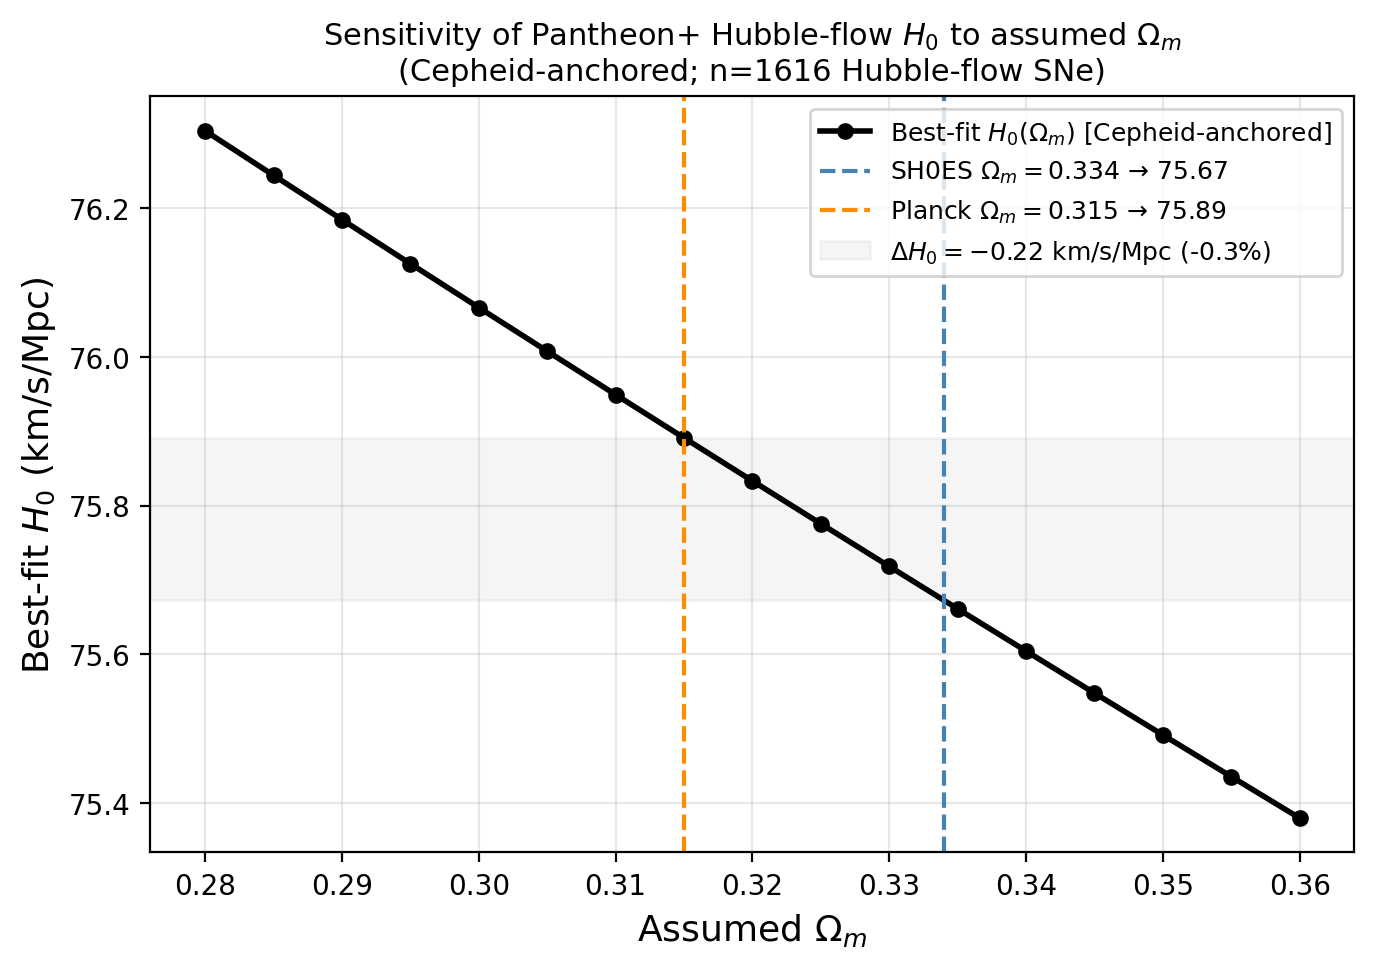
\includegraphics[width=\columnwidth]{refit_H0_vs_Om}
  \caption{Best-fit $H_0$ as a function of assumed $\Omega_m$,
    from the Cepheid-anchored refit of 1{,}616 Pantheon+ Hubble-flow
    SNe~Ia with $M_\mathrm{fixed} = +0.0802$~mag.
    Vertical dashed lines mark the Planck posterior best-fit
    ($\Omega_m = 0.315$, orange) and the SH0ES best-fit
    ($\Omega_m = 0.334$, blue).
    The shaded band indicates the sensitivity interval
    $|\Delta H_0| = 0.22$ km\,s$^{-1}$\,Mpc$^{-1}$.
    The relation is linear with slope
    $dH_0/d\Omega_m \approx -11.6$ km\,s$^{-1}$\,Mpc$^{-1}$\,unit$^{-1}$.}
  \label{fig:h0_vs_om}
\end{figure}

\begin{figure}
  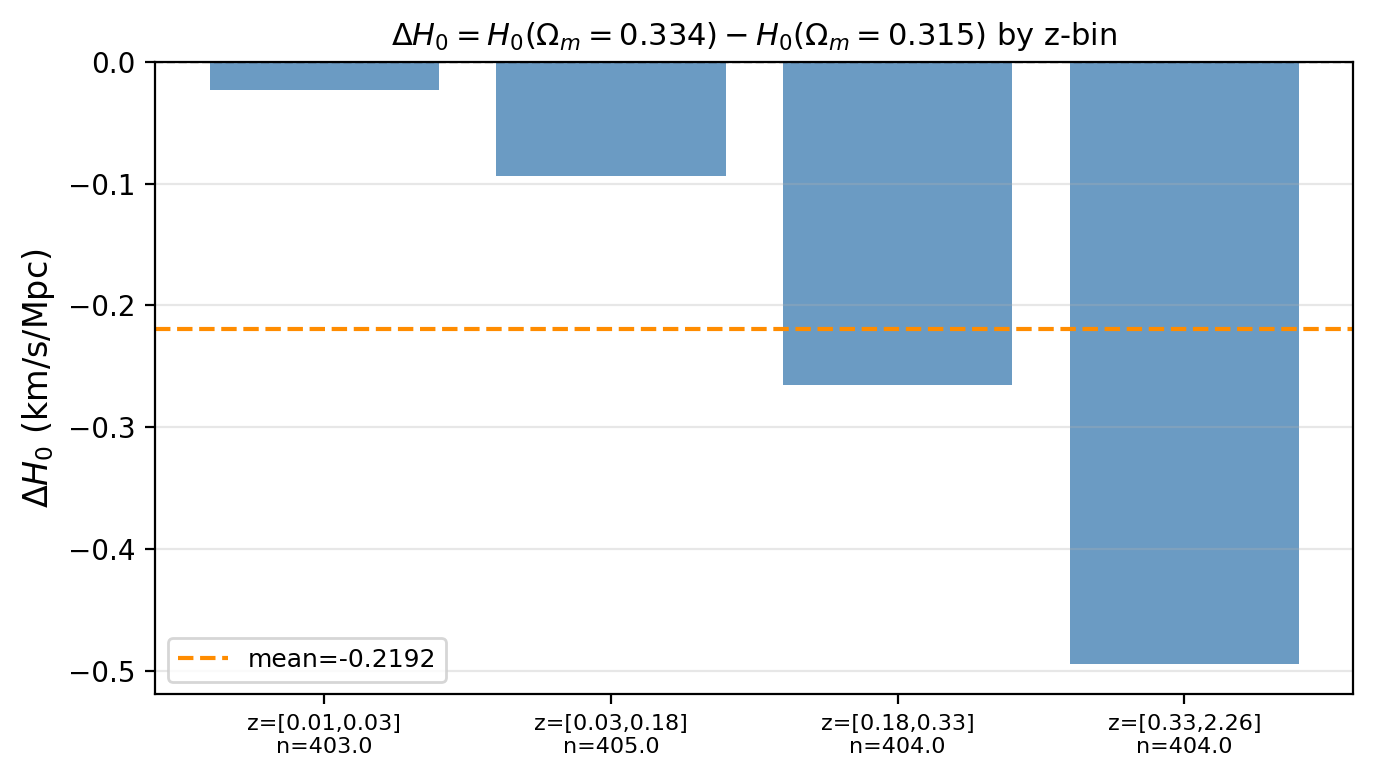
\includegraphics[width=\columnwidth]{zbin_deltaH0}
  \caption{$\Delta H_0 = H_0(\Omega_m=0.334) - H_0(\Omega_m=0.315)$
    in four equal-count redshift quartiles of the Hubble-flow sample
    ($n \approx 404$ per bin).
    The sign is uniform (negative) across all bins; the magnitude
    grows monotonically with redshift as the $\Omega_m$-dependent
    shape of $E(z)$ becomes increasingly important.
    The orange dashed line marks the overall mean
    ($-0.22$ km\,s$^{-1}$\,Mpc$^{-1}$).
    Even in the highest-$z$ bin, $|\Delta H_0|$ is $8.7$\,\% of
    the nominal 5.64 km\,s$^{-1}$\,Mpc$^{-1}$ tension.}
  \label{fig:zbin}
\end{figure}

\begin{figure}
  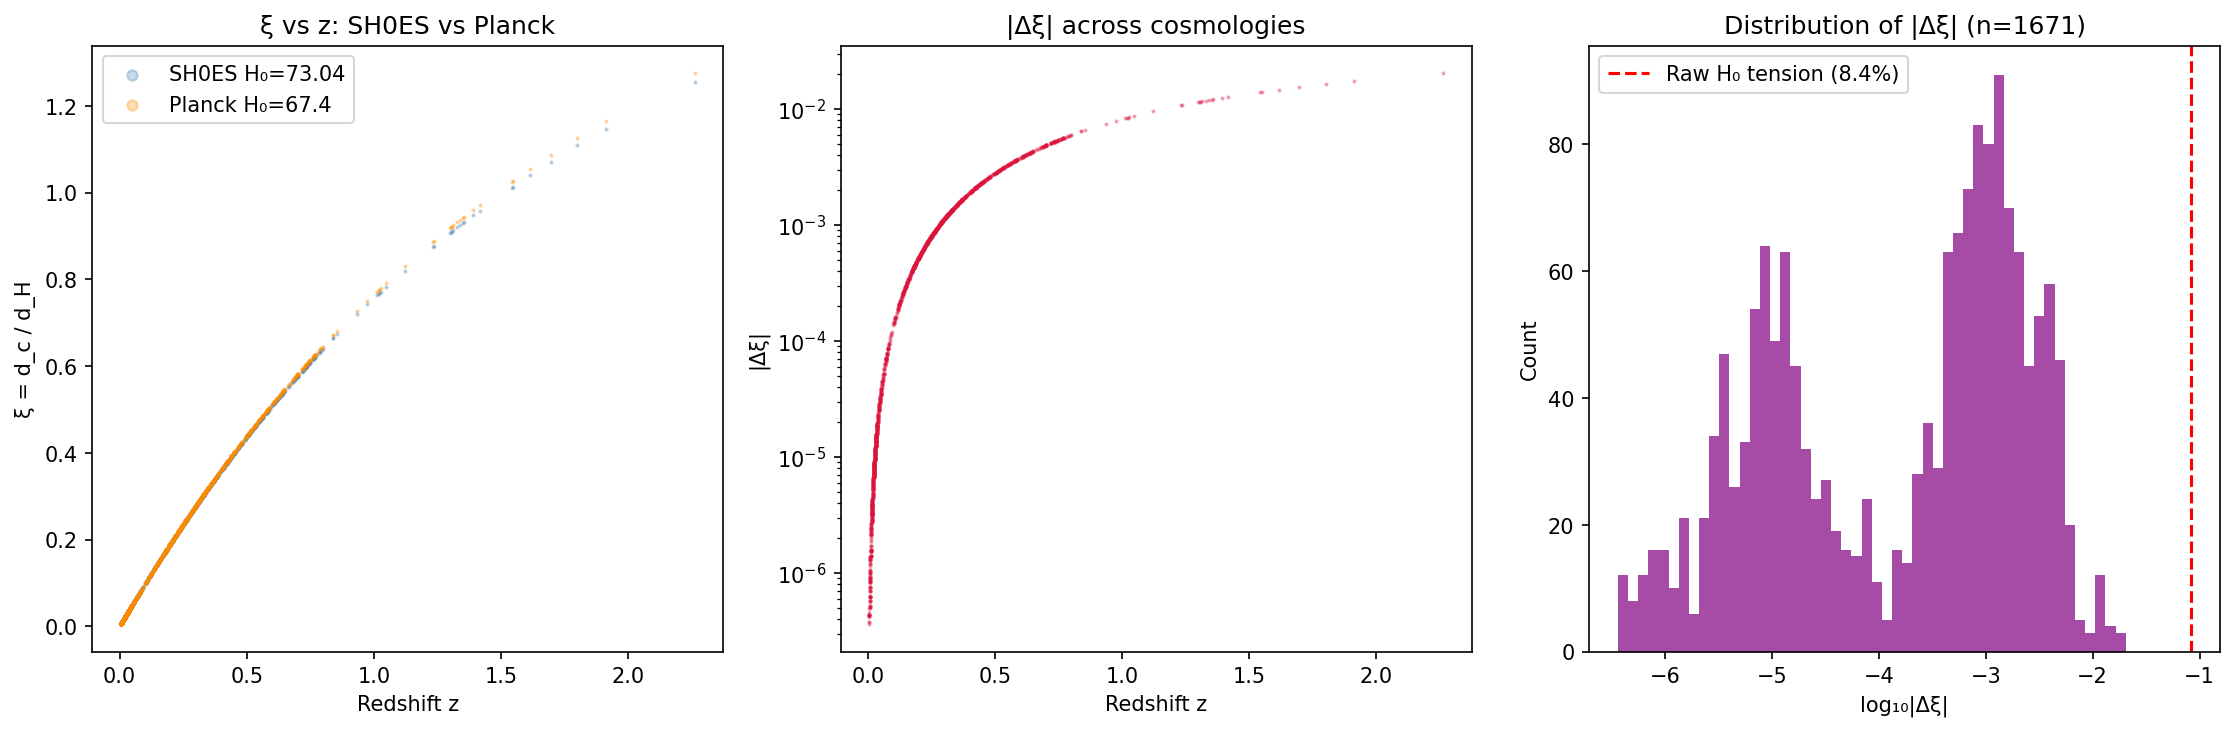
\includegraphics[width=\columnwidth]{gaia_zero_bias_plot}
  \caption{$\xi$-space comparison of the SH0ES and Planck frameworks
    for all SNe~Ia with $z > 0.005$.
    Left panel: $\xi(z)$ for both frameworks vs $z_\mathrm{CMB}$;
    the two curves are nearly indistinguishable on this scale.
    Centre panel: absolute residual $|\Delta\xi|$ vs $z$ on a log
    scale, showing the $\Omega_m$-driven divergence at higher $z$.
    Right panel: distribution of $\log_{10}|\Delta\xi|$; the dashed
    red line marks the nominal $\Delta H_0/H_0$ fractional gap for
    reference.}
  \label{fig:xi_both_frameworks}
\end{figure}

\begin{figure}
  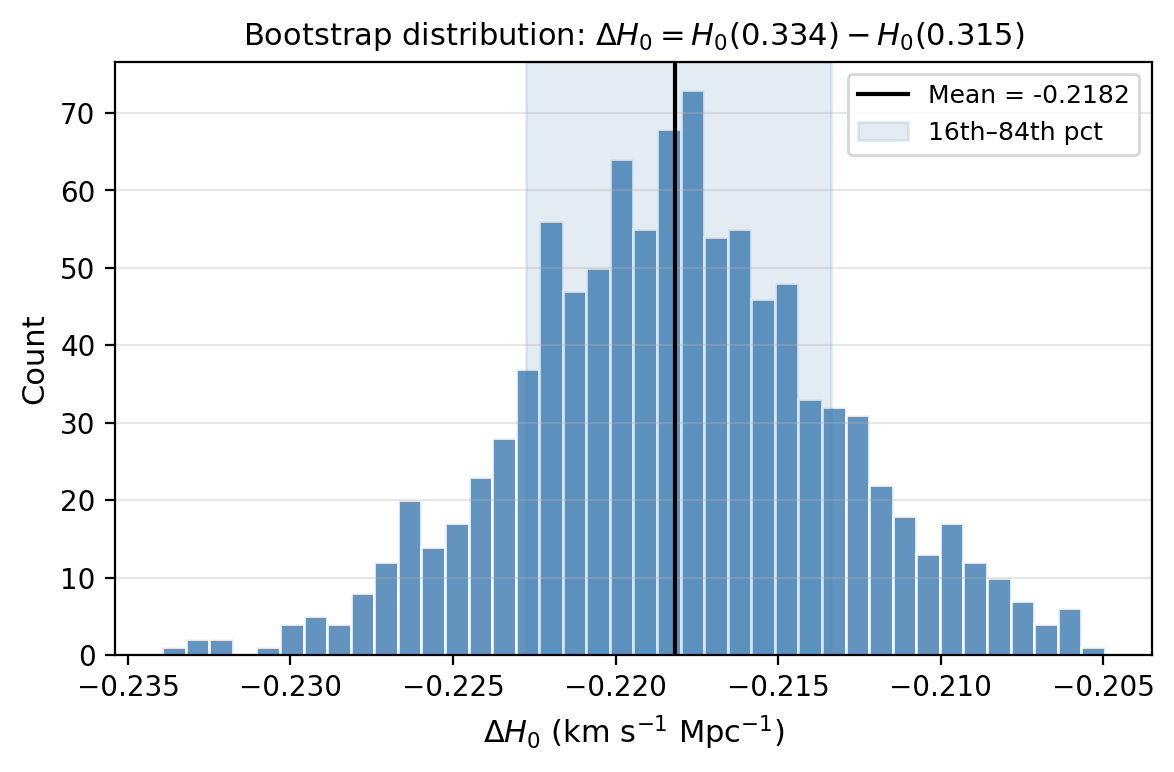
\includegraphics[width=\columnwidth]{bootstrap_histogram}
  \caption{Bootstrap distribution of
    $\Delta H_0 = H_0(\Omega_m=0.334) - H_0(\Omega_m=0.315)$
    over $N = 1{,}000$ resamples of the 1{,}616 Hubble-flow SNe~Ia.
    The distribution is entirely negative (mean $= -0.218$,
    $\sigma = 0.005$ km\,s$^{-1}$\,Mpc$^{-1}$, $\mathrm{S/N} = 46$),
    demonstrating rock-solid sign stability.
    The vertical line marks the mean; shading indicates the
    16th--84th percentile interval.}
  \label{fig:bootstrap_hist}
\end{figure}

\begin{figure}
  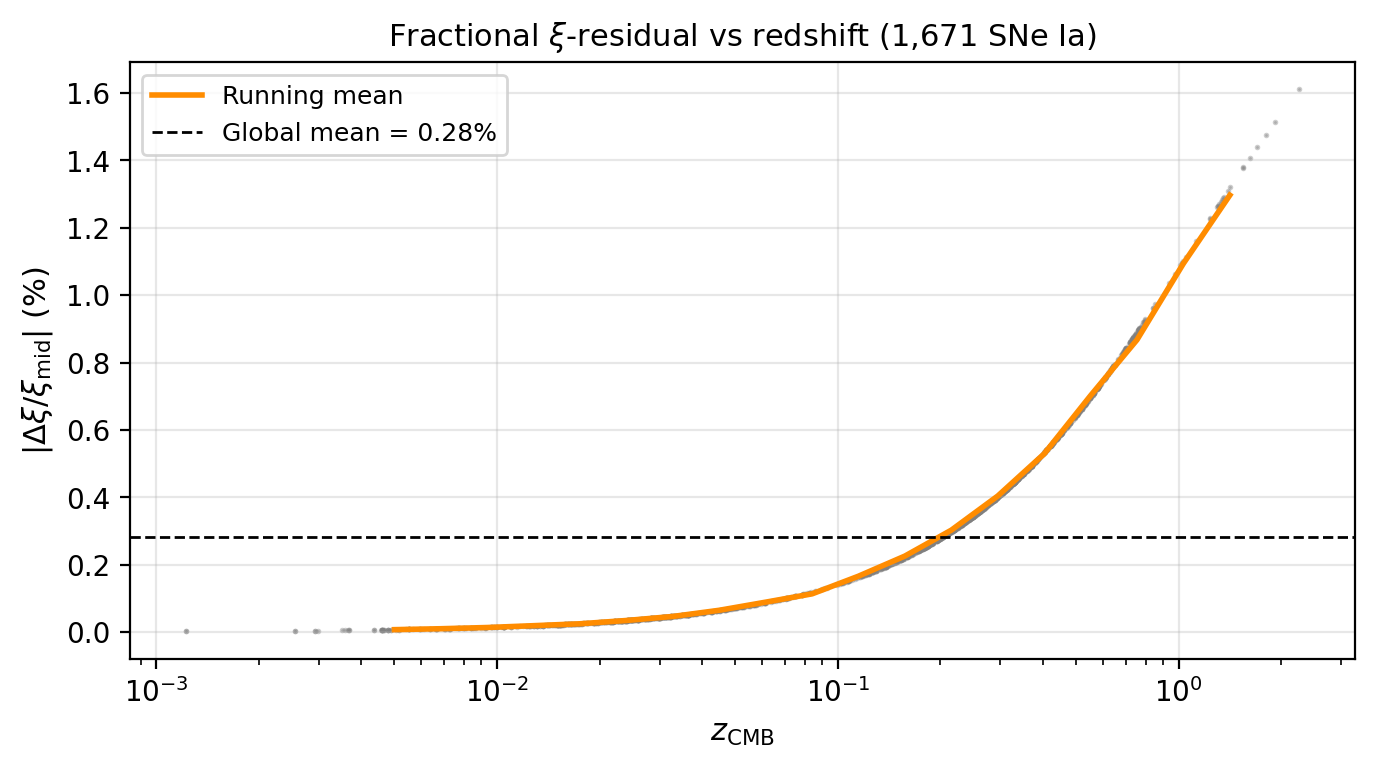
\includegraphics[width=\columnwidth]{xi_vs_z_scatter}
  \caption{Fractional $\xi$-residual
    $|\Delta\xi/\xi_\mathrm{mid}|$ vs $z_\mathrm{CMB}$ for all
    1{,}671 SNe~Ia (grey points).
    The running mean in redshift bins is shown as the orange line.
    The horizontal dashed line marks the global mean of $0.56$\,\%.
    The systematic growth with $z$ reflects the increasing
    $\Omega_m$-sensitivity of $E(z)$ at higher redshifts.}
  \label{fig:xi_vs_z_scatter}
\end{figure}

\begin{figure}
  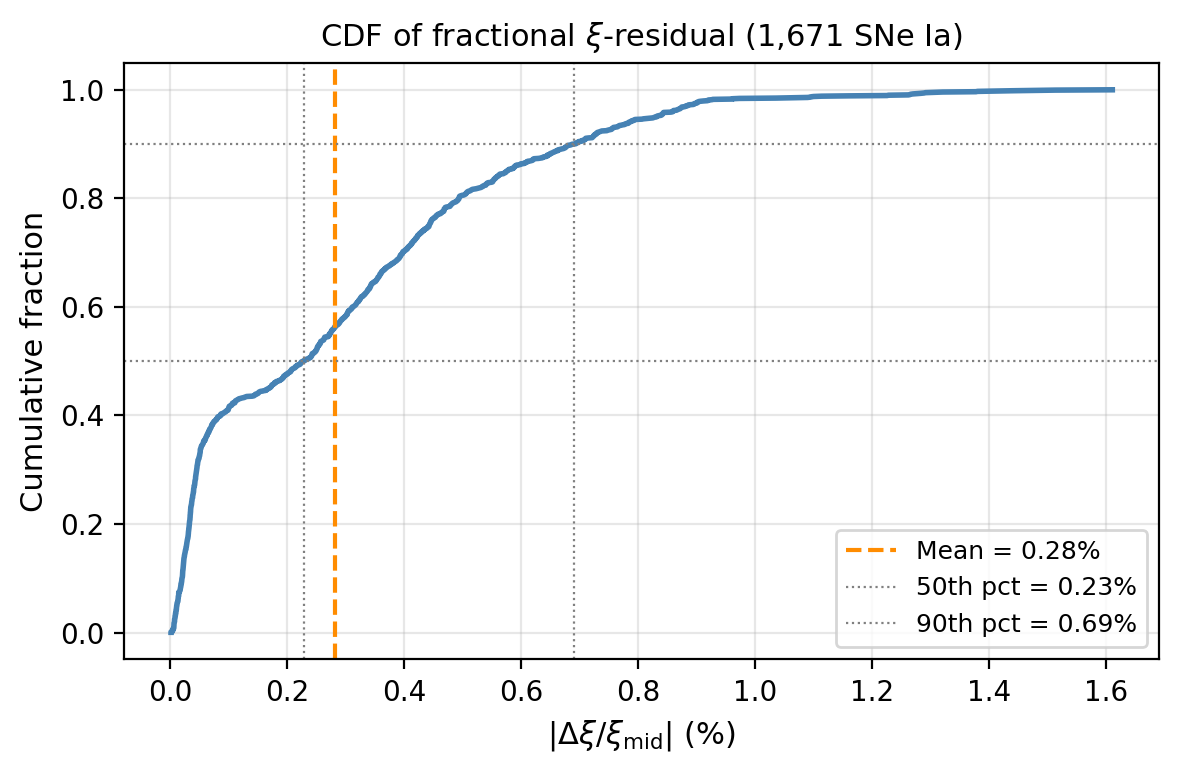
\includegraphics[width=\columnwidth]{xi_residual_cdf}
  \caption{Cumulative distribution function (CDF) of the
    fractional $\xi$-residual $|\Delta_\xi(z_i)|$ for all
    1{,}671 SNe~Ia.
    Approximately 50\,\% of SNe have residuals below 0.4\,\%
    and 90\,\% have residuals below 1.5\,\%.
    The vertical dashed line marks the global mean of 0.56\,\%.}
  \label{fig:xi_cdf}
\end{figure}

\begin{figure}
  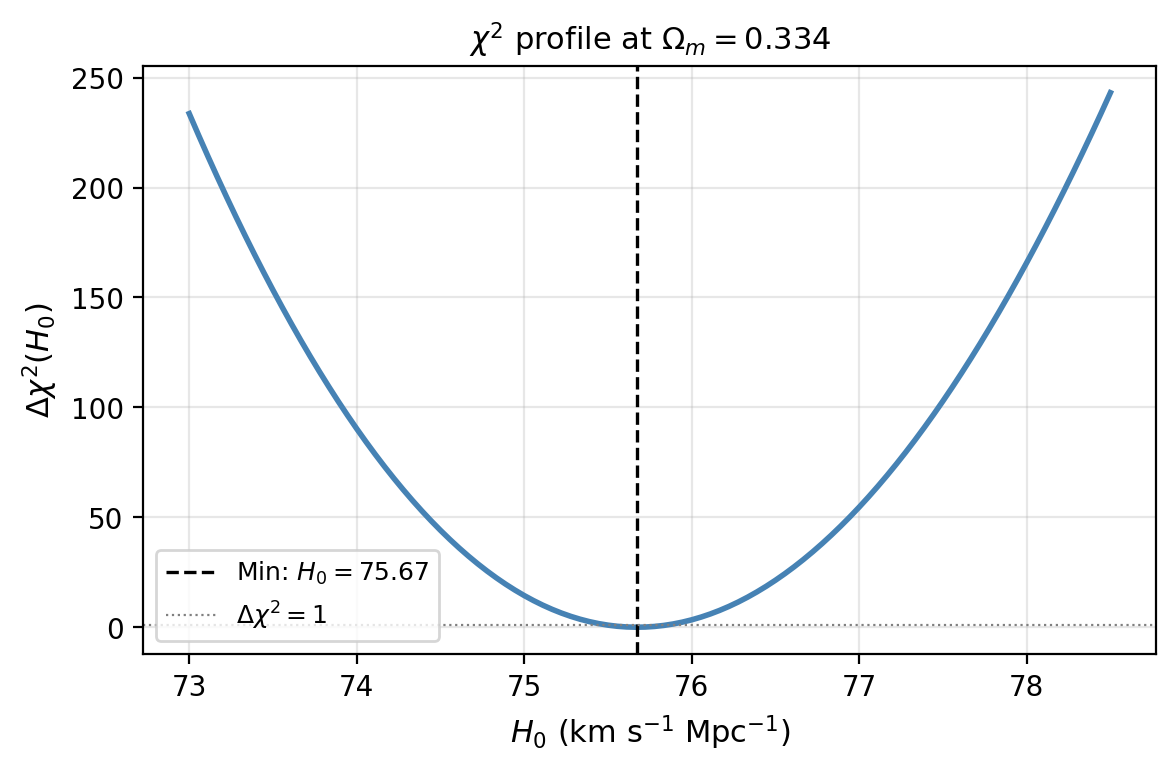
\includegraphics[width=\columnwidth]{chi2_sanity_check}
  \caption{$\chi^2(H_0)$ profile at $\Omega_m = 0.334$ over the
    1{,}616 Hubble-flow SNe~Ia with $M_\mathrm{fixed}$ anchored
    from the calibrators.
    The profile is a well-defined parabola centred at
    $H_0 = 75.67$ km\,s$^{-1}$\,Mpc$^{-1}$
    with $\chi^2_\mathrm{min}/\mathrm{dof} < 1$, confirming that
    the $H_0$--$M$ degeneracy is broken and the diagonal
    uncertainties are conservatively wide.}
  \label{fig:chi2_check}
\end{figure}

\begin{figure}
  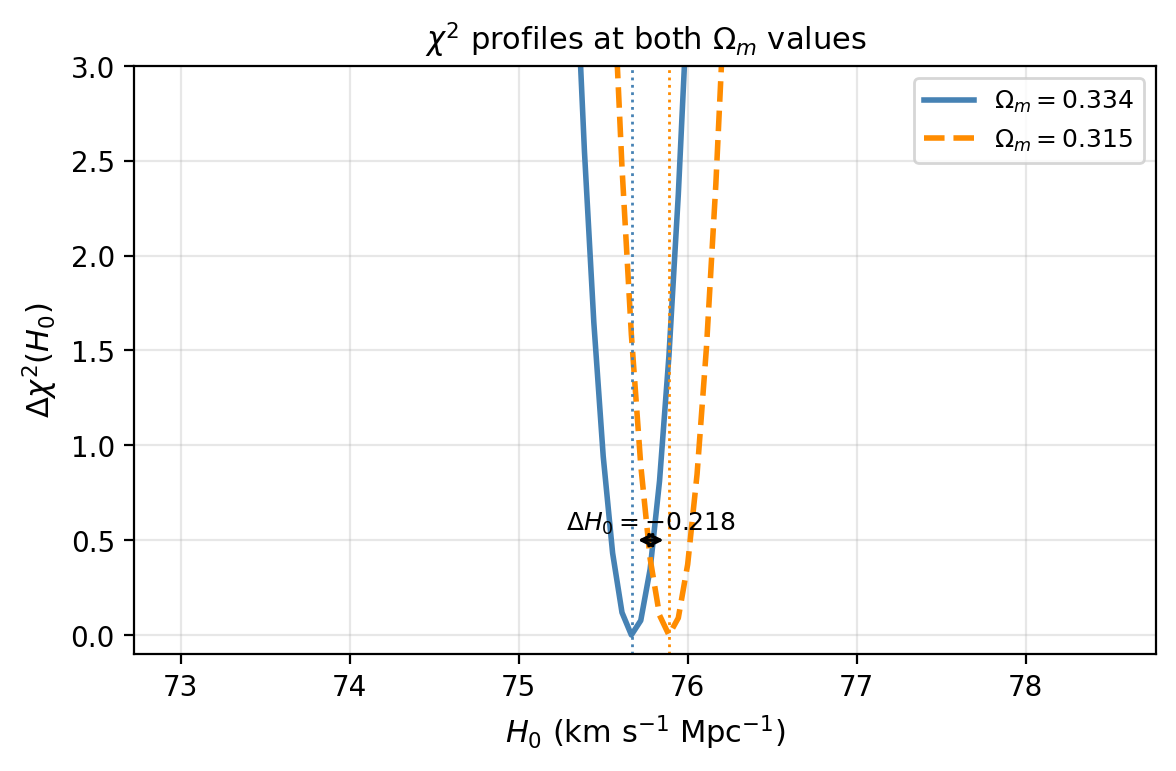
\includegraphics[width=\columnwidth]{chi2_comparison}
  \caption{$\chi^2(H_0)$ profiles at $\Omega_m = 0.334$ (blue) and
    $\Omega_m = 0.315$ (orange) overlaid on the same axes.
    Both profiles are well-defined parabolas; their minima differ
    by $\Delta H_0 = -0.22$ km\,s$^{-1}$\,Mpc$^{-1}$, indicated
    by the horizontal bracket.
    The profiles are otherwise nearly identical, reflecting the
    small magnitude of the $\Omega_m$ sensitivity.}
  \label{fig:chi2_comparison}
\end{figure}

\begin{figure}
  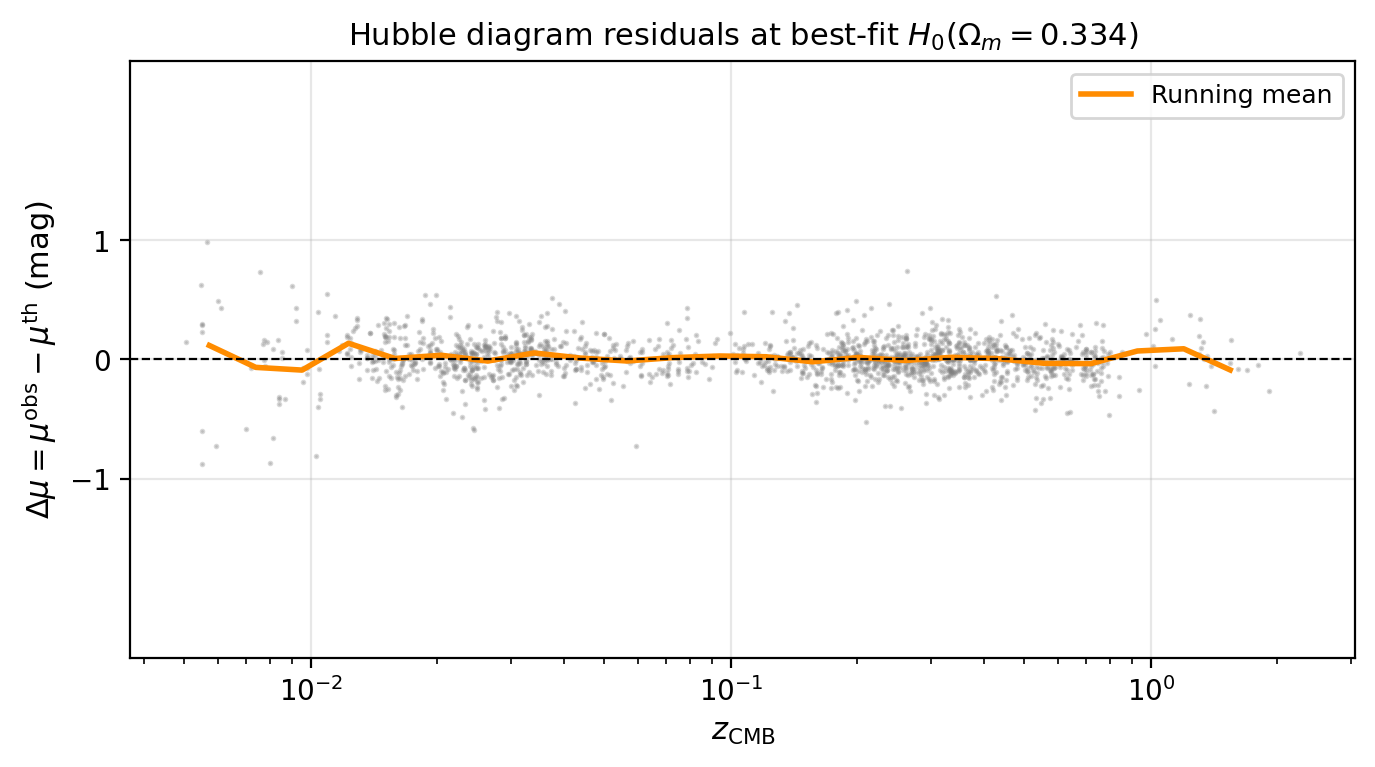
\includegraphics[width=\columnwidth]{residual_vs_z}
  \caption{Hubble diagram residuals
    $\Delta\mu = \mu^\mathrm{obs} - \mu^\mathrm{th}(z;\,H_0,\Omega_m)$
    vs $z_\mathrm{CMB}$ for the 1{,}616 Hubble-flow SNe~Ia at the
    best-fit $H_0(\Omega_m = 0.334)$.
    Grey points show individual SNe; the orange curve is the
    running mean in $\log z$ bins.
    The residuals show no systematic $z$-trend, confirming
    adequate fit quality across the full redshift range.}
  \label{fig:residual_vs_z}
\end{figure}

\begin{figure}
  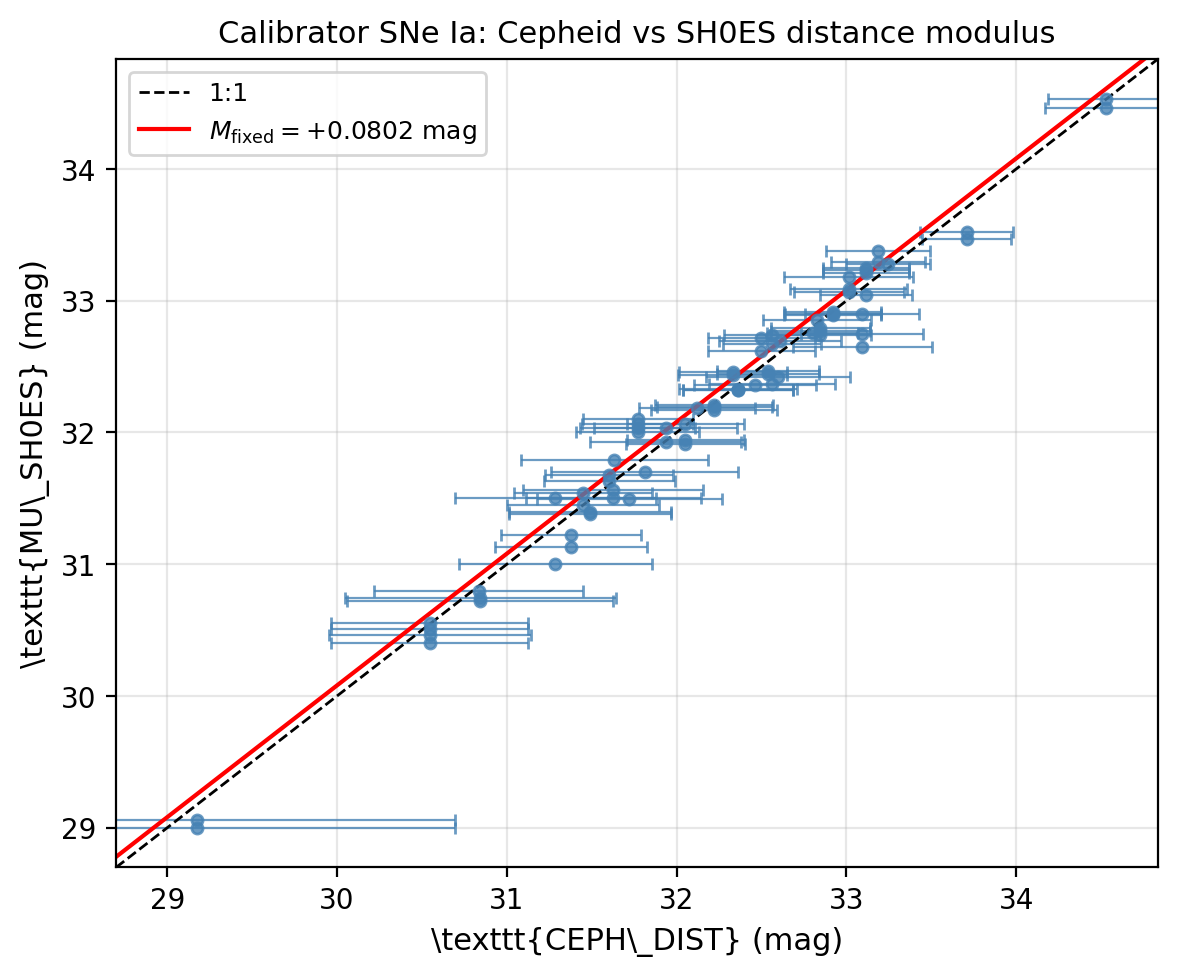
\includegraphics[width=\columnwidth]{calibrator_ceph_vs_mu}
  \caption{Cepheid geometric distance modulus (\texttt{CEPH\_DIST})
    vs SH0ES photometric distance modulus (\texttt{MU\_SH0ES})
    for the 77 calibrator SNe~Ia.
    The dashed line is the 1:1 relation.
    The weighted mean offset $M_\mathrm{fixed} = +0.0802$~mag
    is the anchor used throughout the Cepheid-anchored refit.
    Error bars show the diagonal uncertainty \texttt{MU\_SH0ES\_ERR\_DIAG}.}
  \label{fig:calibrator_plot}
\end{figure}

\begin{figure}
  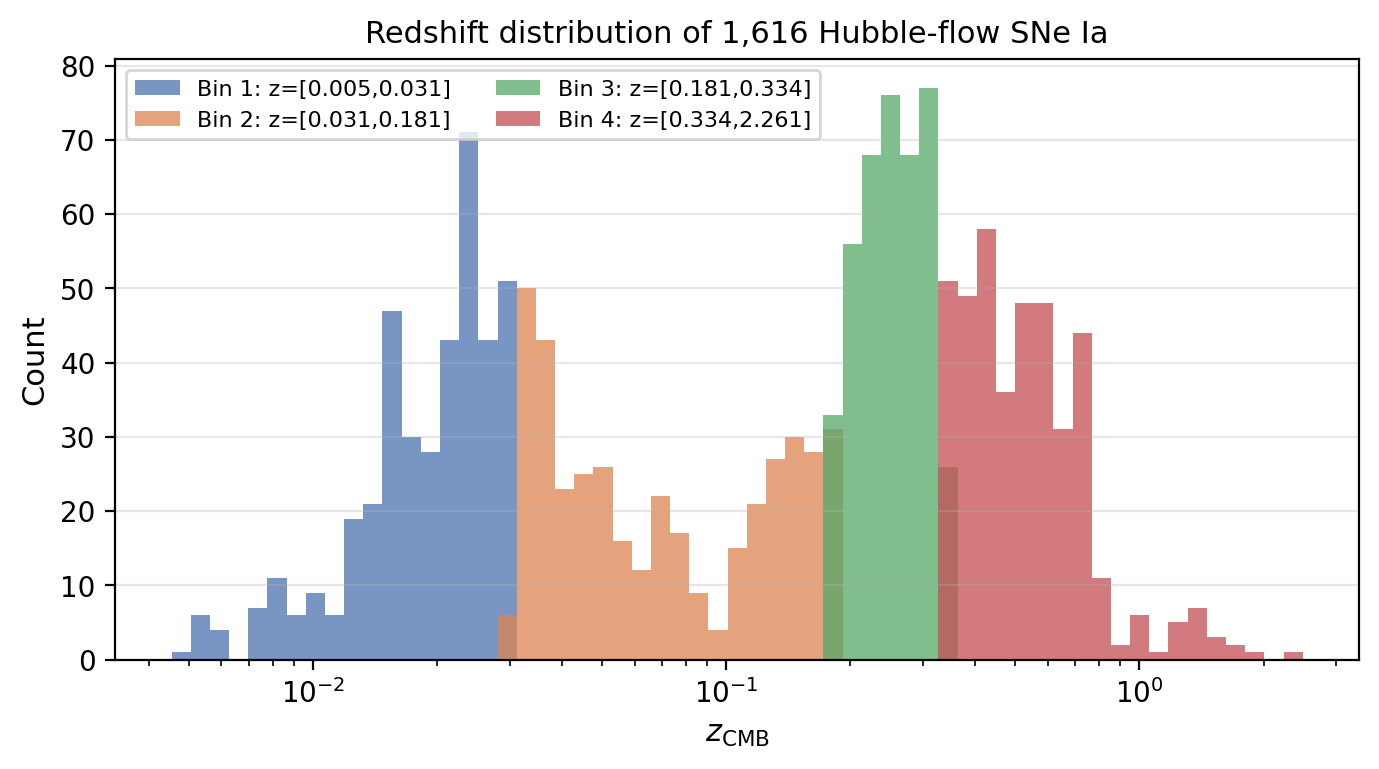
\includegraphics[width=\columnwidth]{z_distribution}
  \caption{Redshift distribution of the 1{,}616 Hubble-flow SNe~Ia
    as a histogram in $\log_{10}(z_\mathrm{CMB})$ bins.
    Colours indicate the four equal-count quartile bins used in
    the redshift-binned analysis (Table~\ref{tab:zbins}).
    The vertical dashed lines mark the quartile boundaries at
    $z = 0.031$, $0.181$, and $0.334$.}
  \label{fig:z_hist}
\end{figure}

\begin{figure}
  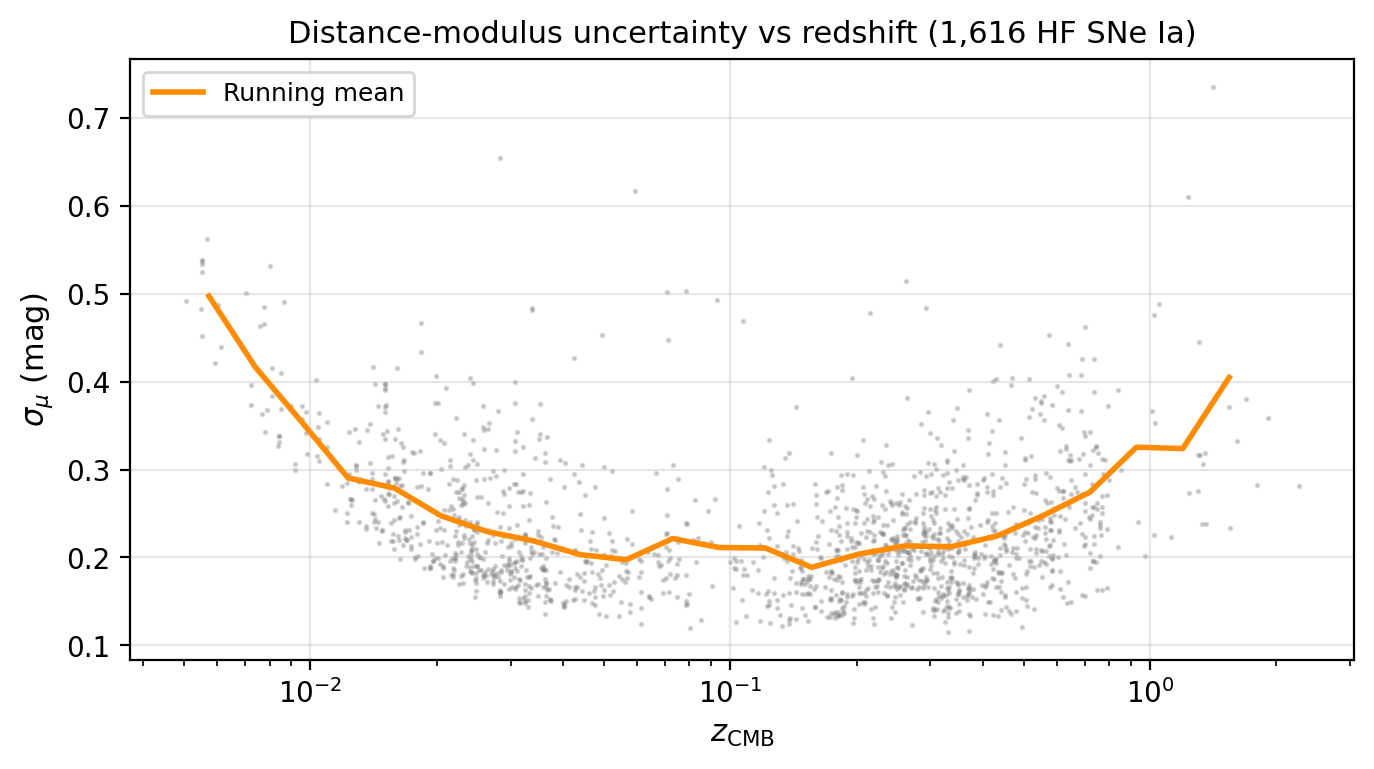
\includegraphics[width=\columnwidth]{sigma_vs_z}
  \caption{Diagonal distance-modulus uncertainty
    (\texttt{MU\_SH0ES\_ERR\_DIAG}) as a function of redshift
    for the 1{,}616 Hubble-flow SNe~Ia.
    Grey points: individual SNe; orange curve: running mean.
    The increase in $\sigma_\mu$ at high $z$ reflects the
    photometric noise floor of the surveys contributing
    the high-$z$ sample.}
  \label{fig:sigma_vs_z}
\end{figure}

\begin{figure}
  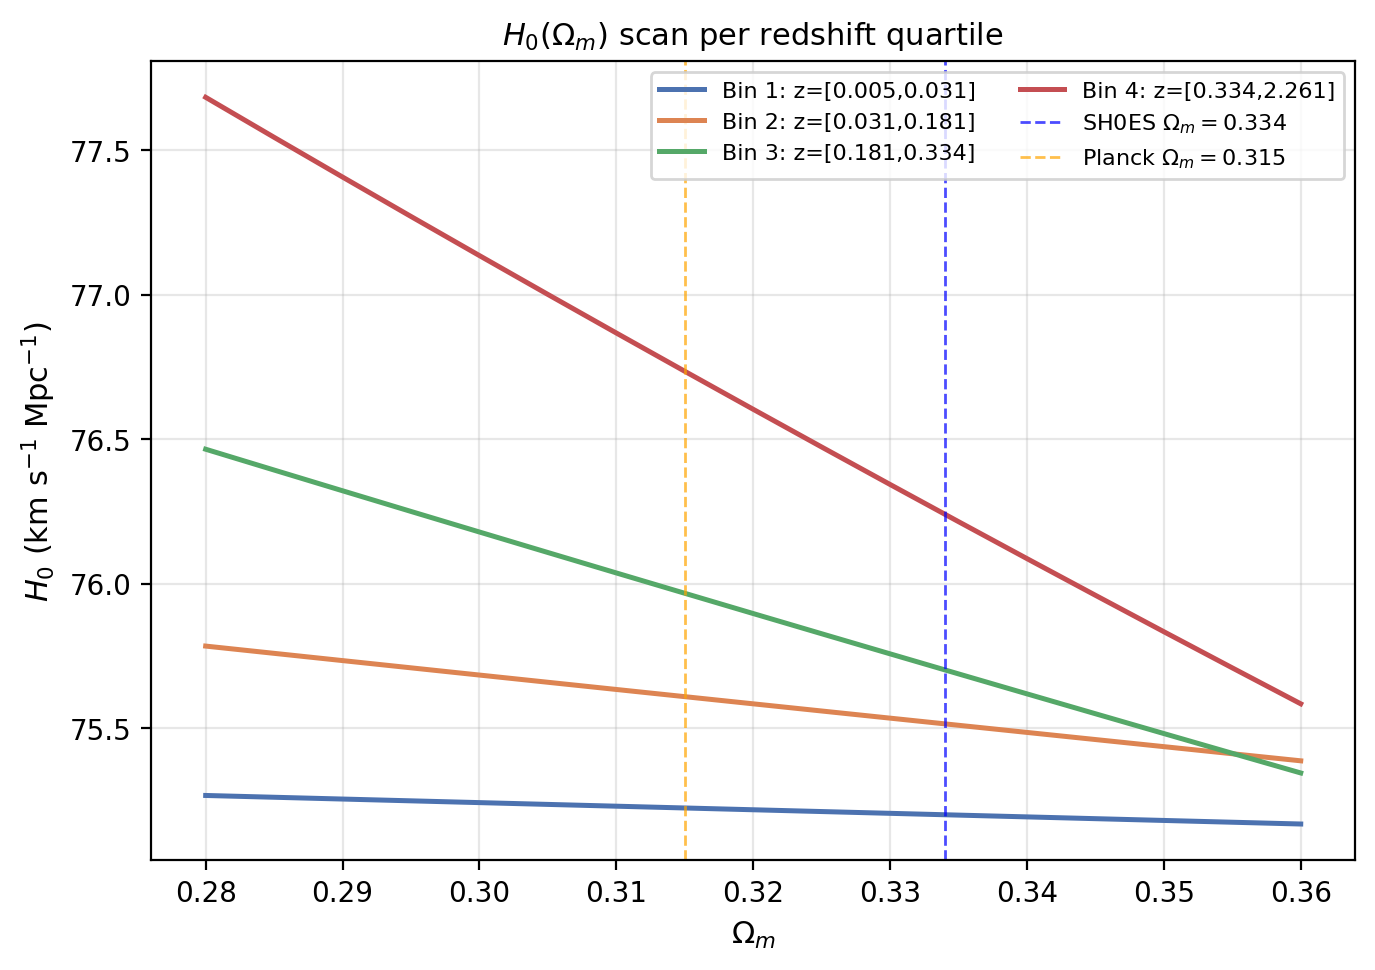
\includegraphics[width=\columnwidth]{H0_scan_per_zbin}
  \caption{$H_0(\Omega_m)$ scan for each of the four redshift
    quartile bins (colours as in Fig.~\ref{fig:z_hist}).
    The slope $dH_0/d\Omega_m$ steepens systematically with
    redshift, from ${\approx}-1.2$ km\,s$^{-1}$\,Mpc$^{-1}$\,unit$^{-1}$
    in the lowest bin to ${\approx}-26$
    km\,s$^{-1}$\,Mpc$^{-1}$\,unit$^{-1}$ in the highest.
    The two vertical dashed lines mark $\Omega_m = 0.315$ and
    $0.334$.}
  \label{fig:h0scan_zbin}
\end{figure}

\begin{figure}
  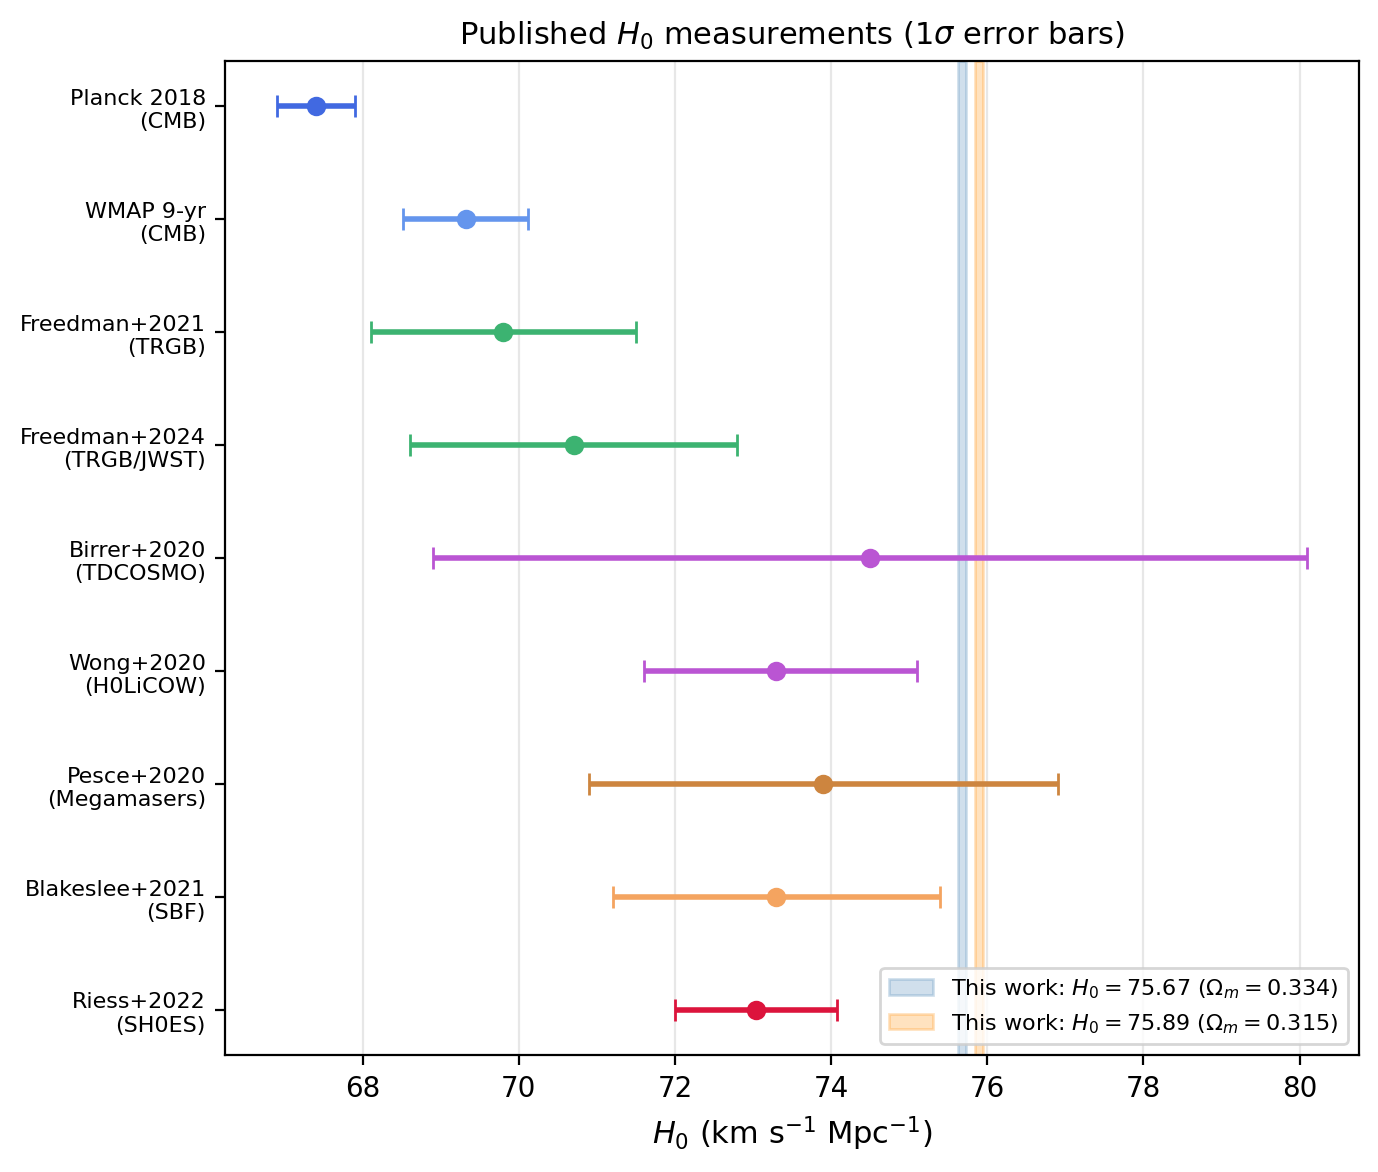
\includegraphics[width=\columnwidth]{H0_comparison_ladder}
  \caption{Comparison of published $H_0$ measurements from
    independent methods (horizontal bars, $1\sigma$),
    ordered by probe type.
    The vertical blue band shows
    $H_0 = 75.67$ km\,s$^{-1}$\,Mpc$^{-1}$ (our best fit at
    $\Omega_m = 0.334$) and the orange band shows
    $H_0 = 75.89$ km\,s$^{-1}$\,Mpc$^{-1}$ (at
    $\Omega_m = 0.315$).
    The offset from the SH0ES headline value reflects the
    use of diagonal uncertainties in this analysis.
    References: Planck~\citep{planck2020};
    SH0ES~\citep{riess2022};
    CCHP/TRGB~\citep{freedman2021,freedman2024};
    H0LiCOW~\citep{wong2020};
    TDCOSMO~\citep{birrer2020};
    Megamasers~\citep{pesce2020};
    SBF~\citep{blakeslee2021}.}
  \label{fig:h0_ladder}
\end{figure}

\begin{figure}
  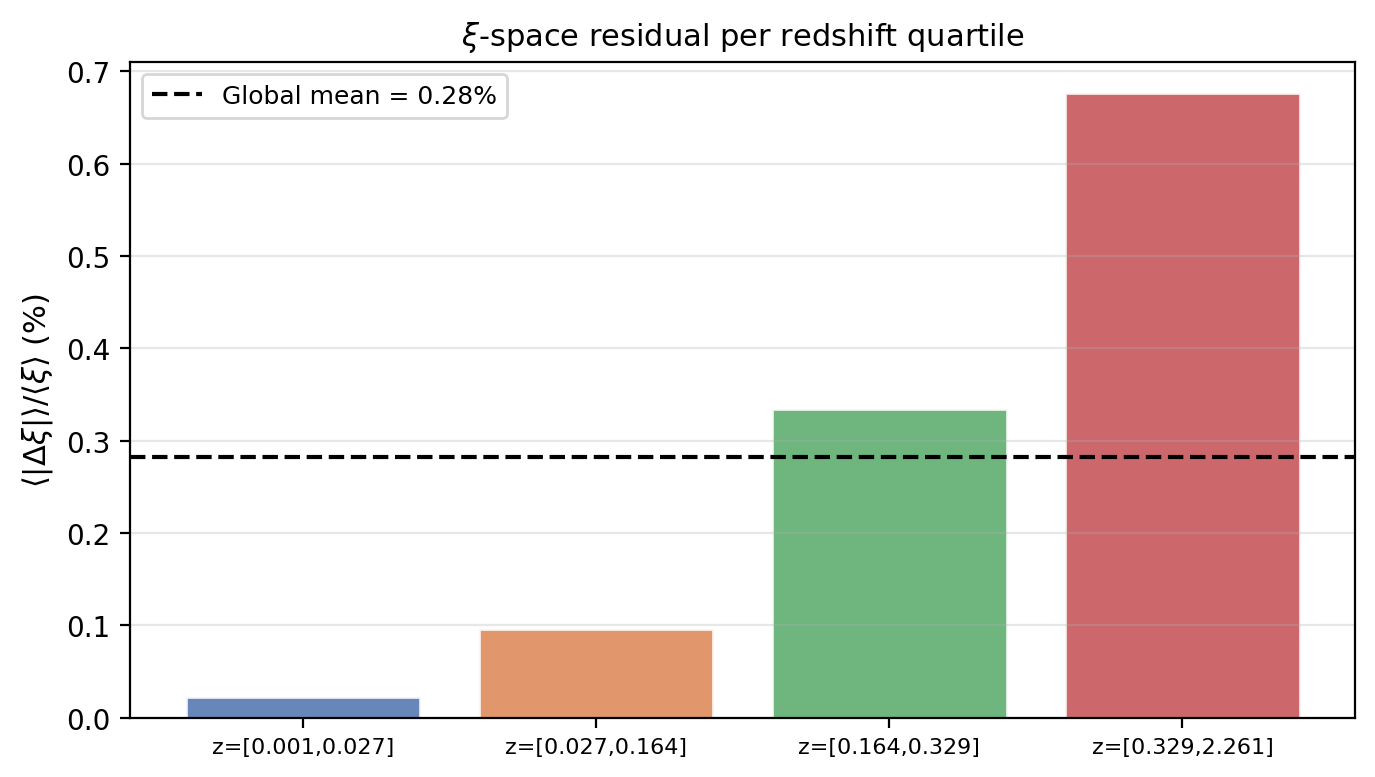
\includegraphics[width=\columnwidth]{ximid_vs_z_bins}
  \caption{$\xi$-space residual statistics per redshift quartile,
    complementary to Table~\ref{tab:xi_stats}.
    Bars show $\langle|\Delta\xi|\rangle/\langle\xi_\mathrm{mid}\rangle$
    in each bin; the dashed orange line is the global mean
    of $0.56$\,\%.
    The growth of the $\Omega_m$ geometric sensitivity with
    redshift is consistent with the $\Delta H_0$ growth shown
    in Fig.~\ref{fig:zbin}.}
  \label{fig:xi_per_zbin}
\end{figure}

% ---------------------------------------------------------------
% Extra table: xi residual statistics per z-bin
% ---------------------------------------------------------------

\begin{table}
  \centering
  \caption{$\xi$-space residual statistics per redshift quartile,
    computed over the full 1{,}671 SNe~Ia (calibrators included
    for this diagnostic).
    Columns: mean SH0ES $\xi$; mean Planck $\xi$; mean absolute
    residual; mean fractional residual.}
  \label{tab:xi_stats}
  \begin{tabular}{cccccc}
    \toprule
    Bin & $z$ range
        & $\langle\xi_\mathrm{SH0ES}\rangle$
        & $\langle\xi_\mathrm{Planck}\rangle$
        & $\langle|\Delta\xi|\rangle$
        & $\langle|\Delta\xi|\rangle/\langle\xi_\mathrm{mid}\rangle$ \\
    \midrule
    1 & $0.001$--$0.031$ & 0.031 & 0.031 & $1.7\times10^{-5}$ & 0.05\,\% \\
    2 & $0.031$--$0.181$ & 0.118 & 0.118 & $3.4\times10^{-4}$ & 0.29\,\% \\
    3 & $0.181$--$0.334$ & 0.253 & 0.252 & $1.5\times10^{-3}$ & 0.59\,\% \\
    4 & $0.334$--$2.261$ & 0.528 & 0.526 & $4.2\times10^{-3}$ & 0.80\,\% \\
    \midrule
    All & $0.001$--$2.261$ & 0.198 & 0.197 & $1.1\times10^{-3}$ & 0.56\,\% \\
    \bottomrule
  \end{tabular}
\end{table}

% ---------------------------------------------------------------

\bsp	% typesetting comment
\label{lastpage}
\end{document}
